% !TeX program = pdflatex
% !TeX spellcheck = en_GB
% !TeX encoding = UTF-8
% !BIB program = biber

% v1.10 - 2017-05-30
% - Erik: Refactor the file structure of the front pages
% - Erik: Fix double bibliography entry
% v1.9 - 2017-02-03
% - Dirk: fixed warning: Underfull \hbox (badness 10000) in paragraph main.tex
% - Dirk: fixed warning: "Data encoding is UTF8" -> style.tex 0.1.8
% v1.8 - 2017-02-02
% - Dirk: replaced titlesec package by KOMA-script commands.-> style.tex v0.1.7
% v1.7 - 2014-11-18
% - bib fixes: now using biber instead of bibtex (thanks felix)
% - compile now with pdflatex -> biber -> pdflatex
% v1.6 - 2013-05-13
% - bibliography headers fixed - thanx lorenz lehmann
% - high quality titlepage - thanx thomas graf
% - removed separation of online and offline references -> style 1.4a
% v1.5 - 2013-01-16

\documentclass[twoside,11pt,titlepage,a4paper,english,bibliography=totocnumbered,listof=numbered]{scrbook}

%--------------------------------------------------------------
% DOCUMENT VARIABLES
%--------------------------------------------------------------

\newcommand{\projectName}{Blockchain-Identity}
\newcommand{\projectVersion}{1.0.0}

%
% Template Style
% =========================================================================
% = SNET THESIS TEMPLATE STYLE
% =========================================================================

% http://www.snet.tu-berlin.de
% ------------------------
% Adapted version from http://hci.rwth-aachen.de/karrer_thesistemplate (Thorsten Karrer)
% Further adaptions for http://www.elearn.rwth-aachen.de (Sascha Hoellger)
% Further adaptions for SNET @ TU Berlin by Sebastian Göndör (sebastian.goendoer@tu-berlin.de)


% =========================================================================
% = CHANGELOG
% =========================================================================
% [0.1.9]
% - Fixed styling for chapters and toc using Komascript
% - Remove double bibliography TOC entry
%
% [0.1.8]
% - fixed "warning UFT8 is used". biblatex requires ascii encoding; by Dirk
%
% [0.1.7]
% replaced "Titelsec" commands (and whole package) by appropriate KOMA-Script commands; by Dirk
%
% [0.1.6]
% replaced deprecated \rm commands with \rmfamily commands; by Dirk
%
% [0.1.4b]
% backend=biber added in line 139
%
% [0.1.4a]
% title page: image logo sizes and margins adjusted to printable area
% removed separation of online and offline references
%
% [0.1.3]
% wider text body
% added "school" to the titlepage
% paragraph indents
% correctly placed footnote graphics
%
% [0.1.2]
% new titlepage
% some minor fixes
%
% [0.1.1]
% changed titlepage logo
% added listoffigures and listoftables
% excluded abstract from toc
% no (roman) numbering for frontmatter
%
% [0.1]
% adapted version 0.991b from sascha hoellger @ rwth aachen


% =========================================================================
% = MISC
% =========================================================================

\usepackage{a4wide}					%
\usepackage{verbatim}				%
\usepackage[toc,page]{appendix}			%
\usepackage[withpage]{acronym}			%
\usepackage{amsthm}				% Definitions


% =========================================================================
% = COLORS
% =========================================================================

\usepackage{xcolor}					% Colors
\definecolor{LightBlue}{rgb}{0.55,0.55,1}
\definecolor{DarkBlue}{rgb}{0.2,0.2,0.5}
\definecolor{DarkRed}{rgb}{0.71,0.12,0.07}

% =========================================================================
% = PAGE LAYOUT
% =========================================================================

\usepackage{geometry}
\geometry{inner=3cm, outer=2cm, bottom=4cm}

\newcommand{\setwidesite}				% changes the geometry to have less margin
{
	\fancyhfoffset[LE,RO]{0cm}
	\fancyheadoffset[LO,RE]{0cm}
	\fancyfootoffset[RE]{2cm}
	\newgeometry{inner=2cm, outer=2cm, bottom=4cm}
}

\usepackage{style/noindent}				%do not indent at new paragraphs but add a vertical offset

\setlength{\parindent}{4mm}
\setlength{\parskip}{1.5mm }


% =========================================================================
% = TYPESETTING
% =========================================================================

\usepackage[hyphens]{url}				% url
\usepackage{hyphenat}				% hyphenation. use \hyphenation{}

\righthyphenmin=5
\lefthyphenmin=5


% =========================================================================
% = TABLE OF CONTENTS
% =========================================================================

\setcounter{secnumdepth}{4}
\setcounter{tocdepth}{3}

\addtokomafont{disposition}{\rmfamily}


% =========================================================================
% = FONTS
% =========================================================================

\usepackage{mathpazo}
\usepackage[scaled=.95]{helvet}
\usepackage{courier}


% =========================================================================
% = SYMBOLS
% =========================================================================

%\usepackage{gensymb}
\usepackage{textcomp} 				% for \textmu (non-italic $\mu$)
\makeatletter						% this makes "@" a regular letter


% =========================================================================
% = TABLES
% =========================================================================

\usepackage{tabularx}
\usepackage{booktabs}
\usepackage{multirow}
\usepackage{longtable}				% tables spanning over more than one page

%%\setlength{\fboxsep}{0mm}			% spacing between \fbox border and content

\usepackage{amsmath}				% math fonts
\usepackage{amssymb}				% math symbols
\usepackage{setspace}				% line spacing


% =========================================================================
% = BIBILOGRAPHY
% =========================================================================

\usepackage[style=numeric,natbib=true,backend=biber]{biblatex}

% apparently no effect?
%\renewcommand{\bibsetup}{
%	\markboth{
%		\MakeUppercase{Bibliography}
%	}{}
%}

\ifdefined\bibheadingonline
  \defbibheading{online}{\section*{\bibheadingonline}}
\else
  \defbibheading{online}{\section*{Online References}}
\fi
\ifdefined\bibheadingoffline
  \defbibheading{offline}{\section*{\bibheadingoffline}}
\else
  \defbibheading{offline}{\section*{Printed References}}
\fi

\defbibfilter{online}{%
  \( \type{online} \)}

\defbibfilter{offline}{%
  \( \not \type{online} \)}

\bibliography{Bibliography}


% =========================================================================
% = LANGUAGE & ENCODING
% =========================================================================

\usepackage[english]{babel}				% \usepackage[ngerman]{babel}

\selectlanguage{english}				% \selectlanguage{ngerman}

\usepackage[T1]{fontenc}
\usepackage[utf8]{inputenc}				% can use native umlauts

% \usepackage[babel,german=quotes]{csquotes}	% provides \enquote{Blupp} => "`Blupp"'
\usepackage[babel,english=american]{csquotes}	% provides \enquote{Blupp} => "`Blupp"'

\SetCiteCommand{\parencite}			% Changed for biblatex

\usepackage{units}					% unified way of setting values with units

\usepackage{appendix}


% =========================================================================
% = CODE LISTINGS
% =========================================================================

\usepackage{listings}

% Listings Styles from Max

\definecolor{violet}{cmyk}{0.45,0.97,0.27,0.21}
\definecolor{lstblue}{cmyk}{1,0.80,0,0}
\definecolor{lstgreen}{cmyk}{0.71,0.21,0.65,0.22}
\definecolor{bluegrey}{cmyk}{0.56,0.24,0.11,0.05}
\definecolor{javadoc}{cmyk}{0.88,0.59,0,0}
\definecolor{lstgrey}{cmyk}{0.55,0.44,0.42,0.32}

\lstdefinelanguage{SQL}{
     keywords={},
     keywordstyle=\color{bluegrey}\bfseries,
     morekeywords=[2]{CREATE,TABLE,IF,NOT,EXISTS,NULL,SET,DEFAULT,PRIMARY,KEY,COLLATE,CHARACTER,AUTO_INCREMENT,ENGINE,CHARSET},
     keywordstyle={[2]\color{violet}\bfseries},
     otherkeywords={int,varchar,double,text,tinyint},
     sensitive=false,
     morecomment=[l][\color{lstgreen}]{//},
     morecomment=[s][\color{lstgreen}]{/*}{*/},
     morecomment=[s][\color{javadoc}]{/**}{*/},
     morestring=[b]',
     morestring=[b]"
  }
\lstdefinelanguage{PHP}{
     keywords={},
     keywordstyle=\color{bluegrey}\bfseries,
     morekeywords=[2]{static,function,if,return,pow,sin,cos,asin,min,sqrt,int},
     keywordstyle={[2]\color{violet}\bfseries},
     otherkeywords={@param, @returns, @author, @type, @link, @see},
     sensitive=false,
     morecomment=[l][\color{lstgreen}]{//},
     morecomment=[s][\color{lstgreen}]{/*}{*/},
     morecomment=[s][\color{javadoc}]{/**}{*/},
     morestring=[b]',
     morestring=[b]"
  }
\lstdefinelanguage{JavaScript}{
     keywords={},
     keywordstyle=\color{bluegrey}\bfseries,
     morekeywords=[2]{attributes, class, classend, do, empty, endif, endwhile, fail, function, functionend, if, implements, in, inherit, inout, not, of, operations, out, return, set, then, types, while, use},
     keywordstyle={[2]\color{violet}\bfseries},
     otherkeywords={@param, @returns, @author, @type, @link, @see},
     sensitive=false,
     morecomment=[l][\color{lstgreen}]{//},
     morecomment=[s][\color{lstgreen}]{/*}{*/},
     morecomment=[s][\color{javadoc}]{/**}{*/},
     morestring=[b]',
     morestring=[b]"
  }
\lstdefinelanguage{Java}{
     keywords={},
     keywordstyle=\color{bluegrey}\bfseries,
     morekeywords=[2]{abstract,boolean,break,byte,case,catch,char,class,
      const,continue,default,do,double,else,extends,false,final,
      finally,float,for,goto,if,implements,import,instanceof,int,
      interface,label,long,native,new,null,package,private,protected,
      public,return,short,static,super,switch,synchronized,this,throw,
      throws,transient,true,try,void,volatile,while},
     keywordstyle={[2]\color{violet}\bfseries},
     morekeywords=[3]{@SuppressWarnings, @Capability, @Override},
     keywordstyle={[3]\color{lstgrey}},
     otherkeywords={@param, @return, @returns, @author, @link, @see},
     sensitive,
     morecomment=[l]//,
     morecomment=[s]{/*}{*/},
     morecomment=[s][\color{javadoc}]{/**}{*/},
     morestring=[b]",
     morestring=[b]',
  }[keywords,comments,strings]

% some listings styles from Gregor Aisch
% http://vis4.net/blog/2009/09/noch-mehr-sprach-definitionen-fuer-latex-listings/

\lstdefinelanguage{HTML5} {morekeywords={a, abbr, address, area, article, aside, audio, b, base, bb, bdo, blockquote,  body, br, button, canvas, caption, cite, code, col, colgroup, command, datagrid, datalist, dd, del, details, dialog, dfn, div, dl, dt, em, embed, eventsource, fieldset, figure, footer,  form,  h1, h2,  h3,  h4, h5,  h6,  head,  header,  hr, html,  i, iframe,  img,  input,  ins, kbd,  label,  legend,  li,  link,  mark,  map,  menu,  meta,  meter,  nav,  noscript,  object,  ol,  optgroup,  option,  output,  p,  param,  pre,  progress,  q,  ruby,  rp,  rt,  samp,  script,  section,  select,  small,  source,  span,  strong,  style,  sub,  sup,  table,  tbody,  td,  textarea,  tfoot,  th,  thead,  time,  title,  tr,  ul,  var,  video},
sensitive=false, morecomment=[s]{<!--}{-->}, morestring=[b]", morestring=[d]'}

\lstdefinelanguage{CSS} {morekeywords={azimuth,  background-attachment,  background-color,  background-image,  background-position,  background-repeat,  background,  border-collapse,  border-color,  border-spacing,  border-style,  border-top, border-right, border-bottom, border-left,  border-top-color, border-right-color, border-bottom-color, border-left-color,  border-top-style, border-right-style, border-bottom-style, border-left-style,  border-top-width, border-right-width, border-bottom-width, border-left-width,  border-width,  border,  bottom,  caption-side,  clear,  clip,  color,  content,  counter-increment,  counter-reset,  cue-after,  cue-before,  cue,  cursor,  direction,  display,  elevation,  empty-cells,  float,  font-family,  font-size,  font-style,  font-variant,  font-weight,  font,  height,  left,  letter-spacing,  line-height,  list-style-image,  list-style-position,  list-style-type,  list-style,  margin-right, margin-left,  margin-top, margin-bottom,  margin,  max-height,  max-width,  min-height,  min-width,  orphans,  outline-color,  outline-style,  outline-width,  outline,  overflow,  padding-top, padding-right, padding-bottom, padding-left,  padding,  page-break-after,  page-break-before,  page-break-inside,  pause-after,  pause-before,  pause,  pitch-range,  pitch,  play-during,  position,  quotes,  richness,  right,  speak-header,  speak-numeral,  speak-punctuation,  speak,  speech-rate,  stress,  table-layout,  text-align,  text-decoration,  text-indent,  text-transform,  top,  unicode-bidi,  vertical-align,  visibility,  voice-family,  volume,  white-space,  widows,  width,  word-spacing,  z-index},
sensitive=false, morecomment=[s]{/*}{*/}, morestring=[b]", morestring=[d]'}

\lstdefinelanguage{JavaFX} {morekeywords={abstract, after, and, as, assert, at, attribute, before, bind, bound, break, catch, class, continue, def, delete, else, exclusive, extends, false, finally, first, for, from, function, if, import, indexof, in, init, insert, instanceof, into, inverse, last, lazy, mixin, mod, new, not, null, on, or, override, package, postinit, private, protected, public-init, public, public-read, replace, return, reverse, sizeof, static, step, super, then, this, throw, trigger, true, try, tween, typeof, var, where, while, with },
sensitive=false, morecomment=[l]{//}, morecomment=[s]{/*}{*/}, morestring=[b]", morestring=[d]'}

\lstdefinelanguage{MXML} {morekeywords={mx:Accordion, mx:Box, mx:Canvas, mx:ControlBar, mx:DividedBox, mx:Form, mx:FormHeading, mx:FormItem, mx:Grid, mx:GridItem, mx:GridRow, mx:HBox, mx:HDividedBox, mx:LinkBar, mx:Panel, mx:TabBar, mx:TabNavigator, mx:Tile, mx:TitleWindow, mx:VBox, mx:VDividedBox, mx:ViewStack, mx:Button, mx:CheckBox, mx:ComboBase, mx:ComboBox, mx:DataGrid, mx:DateChooser, mx:DateField, mx:HRule, mx:Image, mx:Label, mx:Link, mx:List, mx:Loader, mx:MediaController, mx:MediaDisplay, mx:MediaPlayback, mx:MenuBar, mx:NumericStepper, mx:ProgressBar, mx:RadioButton, mx:RadioButtonGroup, mx:Spacer, mx:Text, mx:TextArea, mx:TextInput, mx:Tree, mx:VRule, mx:VScrollBar, mx:Application, mx:Repeater, mx:UIComponent, mx:UIObject, mx:View, mx:FlexExtension, mx:UIComponentExtension, mx:UIObjectExtension, mx:Fade, mx:Move, mx:Parallel, mx:Pause, mx:Resize, mx:Sequence, mx:WipeDown, mx:WipeLeft, mx:WipeRight, mx:WipeUp, mx:Zoom, mx:EventDispatcher, mx:LowLevelEvents, mx:UIEventDispatcher, mx:CurrencyFormatter, mx:DateFormatter, mx:NumberFormatter, mx:PhoneFormatter, mx:ZipCodeFormatter, mx:CursorManager, mx:DepthManager, mx:DragManager, mx:FocusManager, mx:HistoryManager, mx:LayoutManager, mx:OverlappedWindows, mx:PopUpManager, mx:SystemManager, mx:TooltipManager, mx:CreditCardValidator, mx:DateValidator, mx:EmailValidator, mx:NumberValidator, mx:PhoneNumberValidator, mx:SocialSecurityValidator, mx:StringValidator, mx:ZipCodeValidator, mx:DownloadProgressBar, mx:ArrayUtil, mx:ClassUtil, mx:Delegate, mx:ObjectCopy, mx:URLUtil, mx:XMLUtil, mx:CSSSetStyle, mx:CSSStyleDeclaration, mx:CSSTextStyles, mx:StyleManager, mx:HTTPService, mx:RemoteObject, mx:Service},
sensitive=false, morecomment=[s]{<!--}{-->}, morestring=[b]", morestring=[d]'}

\lstdefinelanguage{LZX} {morekeywords={a, alert, animator, animatorgroup , attribute, audio , axis, axisstyle , b, barchart, basebutton , basebuttonrepeater , basecombobox , basecomponent , basedatacombobox , basedatepicker , basedatepickerday , basedatepickerweek , basefloatinglist , basefocusview , baseform , baseformitem , basegrid , basegridcolumn , baselist , baselistitem , basescrollarrow , basescrollbar , basescrollthumb , basescrolltrack , baseslider , basestyle , basetab , basetabelement , basetabpane , basetabs , basetabsbar , basetabscontent , basetabslider , basetrackgroup , basetree , basevaluecomponent , basewindow , br , button , canvas , chart , chartbgstyle , chartstyle , checkbox , class , columnchart , combobox , command , connection , connectiondatasource , constantboundslayout , constantlayout , datacolumn , datacombobox , datalabel , datamarker , datapath , datapointer , dataselectionmanager , dataseries , dataset , datasource , datastyle , datastylelist , datatip , datepicker , debug , dragstate , drawview , edittext , event , face , floatinglist , font , font , form , frame , grid , gridcolumn , gridtext , handler , hbox , horizontalaxis , hscrollbar , i , image , img , import , include , inputtext , javarpc , label , labelstyle , layout , legend , library , linechart , linestyle , list , listitem , LzTextFormat , menu , menubar , menuitem , menuseparator , method , modaldialog , multistatebutton , node , p , param , piechart , piechartplotarea , plainfloatinglist , plotstyle , pointstyle , pre , radiobutton , radiogroup , rectangularchart , regionstyle , remotecall , resizelayout , resizestate , resource , reverselayout , richinputtext , rpc , script , scrollbar , security , selectionmanager , sessionrpc , simpleboundslayout , simpleinputtext , simplelayout , slider , soap , splash , stableborderlayout , state , statictext , style , submit , swatchview , SyncTester , tab , tabelement , tabpane , tabs , tabsbar , tabscontent , tabslider , Test , TestCase , TestResult , TestSuite , text , textlistitem , tickstyle , tree , u , valueline , valuelinestyle , valuepoints , valuepointstyle , valueregion , valueregionstyle , vbox , verticalaxis , view , view , vscrollbar , webapprpc , window , windowpanel , wrappinglayout , XMLHttpRequest , xmlrpc , zoomarea},
sensitive=false, morecomment=[s]{<!--}{-->}, morestring=[b]", morestring=[d]'}

\lstset{
  numbers=left,
  numberstyle=\tiny,
  numbersep=5pt,
  breaklines=true,
  stepnumber=1,
  tabsize=2,
  basicstyle=\ttfamily\small,
  frame=none,
  numberfirstline=true,
  firstnumber=1,
  keywordstyle=\color{violet}\bfseries,
  ndkeywordstyle=\color{bluegrey}\bfseries,
  identifierstyle=\color{black},
  commentstyle=\color{lstgreen}\ttfamily,
  stringstyle=\color{lstblue}\ttfamily,
  showstringspaces=false
}


% ========================================================================
% = CHANGE LIST DEFINITIONS
% ========================================================================

% change color of item list
\renewcommand{\labelitemi}{\color{DarkRed}$\bullet$}
\renewcommand{\labelitemii}{\color{DarkRed}$\circ$}
\renewcommand{\labelitemiii}{\color{DarkRed}$\ast$}
\renewcommand{\labelitemiv}{\color{DarkRed}$\diamond$}

% change color of enum list
\renewcommand{\labelenumi}{\color{DarkRed}\arabic{enumi}.}
\renewcommand{\labelenumii}{\color{DarkRed}\alph{enumii})}
\renewcommand{\labelenumiii}{\color{DarkRed}\roman{enumiii}.}
\renewcommand{\labelenumiv}{\color{DarkRed}\Alph{enumiv}.}

% change color of description list
\usepackage{enumitem}
\setdescription{font=\color{DarkRed}\rmfamily\itshape}
% \renewenvironment{description}{\list{font=\color{DarkRed}\itshape}}{\endlist}


% ========================================================================
% = FOOTNOTES
% ========================================================================

% change color of footnotes
\renewcommand{\thefootnote}{\color{DarkRed}\arabic{footnote}}

% use nice footnote indentation
\deffootnote[1em]{1em}{1em}{\textsuperscript{\thefootnotemark}\,}


% =========================================================================
% = GRAPHICS AND IMAGES
% =========================================================================

\usepackage{graphicx}
\graphicspath{{images/}}				% path to your image folder

\usepackage{eso-pic}					% needed for the full-face titlepage
\usepackage{chngpage}				% we need this to determine if a figure is on an odd or even page
\usepackage{tikz}					% tikz pictures

% captions of tables and images
\usepackage[hang,small,sf]{caption}
\renewcommand{\captionfont}{\sffamily\small}
\renewcommand{\captionlabelfont}{\bfseries}

\usepackage{float}
\usepackage{placeins}
% \floatstyle{ruled}
%\floatplacement

\renewcommand{\floatpagefraction}{0.85}		% if a figure takes more than 85% of a page it will be typeset on a separate page
\usepackage[it,bf,tight,hang,raggedright]{subfigure}

%\numberwithin{figure}{section}
%\numberwithin{table}{section}


% =========================================================================
% = HEADER
% =========================================================================

\newcommand{\STYLEfootnotetext}
{
  \begin{minipage}
  {.2\textwidth}
    
\includegraphics[width=0.9\textwidth]{images/snet/snet_footer.png}
  \end{minipage}
}

% Change page headers and footers:
\usepackage{calc}
\usepackage{fancyhdr}
\pagestyle{fancy}
\fancyhfoffset[RO,LE]{0.1cm} %{\marginparsep+\marginparwidth}
\fancyhfoffset[RE,LO]{0.1cm}
%\fancyheadoffset[RE,LO]{\hoffset + \oddsidemargin}
\renewcommand{\headrule}{{\color{DarkRed}%
  \hrule width\headwidth height\headrulewidth \vskip-\headrulewidth}}
\fancyhf{}
\fancyhead[RE]{\slshape \nouppercase{\leftmark}}    % Even page header: "page   chapter"
\fancyhead[LO]{\slshape \nouppercase{\rightmark}}   % Odd  page header: "section   page"
\fancyhead[RO,LE]{\bfseries \thepage}

%- \fancyfoot[LE]{\STYLEleftpicture}
%- \fancyfoot[RO]{\STYLErightpicture}
\fancyfoot[LE]{\STYLEfootnotetext}

\renewcommand{\headrulewidth}{1pt}    % Underline headers
\renewcommand{\footrulewidth}{0pt}

% =========================================================================
% = SECTIONS THEMING
% =========================================================================

\newcommand{\allsectionformat}{\color{DarkRed}\rmfamily\normalfont}

% Font style and colors
\addtokomafont{part}{\Huge\allsectionformat}
\addtokomafont{chapter}{\Huge\allsectionformat}
\addtokomafont{section}{\allsectionformat}
\addtokomafont{subsection}{\allsectionformat}
\addtokomafont{subsubsection}{\allsectionformat}
\addtokomafont{paragraph}{\allsectionformat}
\addtokomafont{subparagraph}{\allsectionformat}

% Spacing before and after the section titles
\RedeclareSectionCommand[
  beforeskip=-.75\baselineskip,
  afterskip=.5\baselineskip]{section}

\RedeclareSectionCommand[
  beforeskip=-5\baselineskip,
  afterskip=.5\baselineskip]{chapter}


% =========================================================================
% = TYPESETTING - TWEAKES
% =========================================================================

\addtokomafont{section}{\LARGE}
\addtokomafont{subsection}{\large}

% instead of sloppy
%\tolerance 1414
%\hbadness 1414
%- \tolerance 2414
%- \hbadness 2414
%- \emergencystretch 1.5em
%- \hfuzz 0.3pt
%- \widowpenalty=10000     % Hurenkinde r
%- \clubpenalty=10000      % Schusterjungen
%- \brokenpenalty=10000
%- \interlinepenalty=9000 % seitenumbruch im absatz
%- \vfuzz \hfuzz
%- \raggedbottom


% =========================================================================
% =  USER DEFINED COMMANDS
% =========================================================================

\newcommand{\chapterquote}[2]{
    \begin{quotation}
    \begin{flushright}
    \noindent\emph{``{#1}''\\[1.5ex]---{#2}}
    \end{flushright}
    \end{quotation}
}

\addbibresource{Bibliography.bib}

% custom hyphenation					
% add words to this list to prevent hyphenation
\hyphenation{
ASCII
TCP
}

%make readable references
\usepackage[pdftex,pdfpagelabels=true]{hyperref}
\hypersetup{%
	pdftitle={\projectName{} \projectVersion{}},
	pdfauthor={Michael Chlepakov, Marvin Petzolt, Timo Runck, Oskar Schlösinger},
	pdfkeywords={key1, key2, key3},
	pdfsubject={Thesis Subject}
}

% Adding a finite stretch on the page suppresses "Underfull \vbox (badness 10000)" warnings.
\makeatletter
\def\@textbottom{\vskip \z@ \@plus 1pt}
\let\@texttop\relax
\makeatother

\begin{document}

%--------------------------------------------------------------
% FRONT PAGE AND DOCUMENT METADATA
%--------------------------------------------------------------
\frontmatter

\begin{titlepage}
	\AddToShipoutPicture*{
		\put(0,0){
			
\includegraphics[width=\paperwidth,height=\paperheight,keepaspectratio=false]{images/snet/titlepage.pdf}
		}
	}
	\strut
	\hfill
	\begin{center}
	\vspace{1cm}
		\Huge
		\begin{spacing}{.9}
			\textcolor{DarkRed}{\textbf{Identity Blockchain}}\\
		\end{spacing}
		\vspace{0.8cm}
		\large
		by\\
		\vspace{0.8cm}
		Michael Chlepakov - 330254 \\
		Marvin Petzolt - 350455 \\
		Timo Runck - 359651 \\
		Oskar Schl{\"o}singer - 347855 \\
		\vspace{2cm}
	 	A documentation submitted to\\
		\vspace{0.5cm}
		Technische Universität Berlin\\
		School IV - Electrical Engineering and Computer Science\\
		Department of Telecommunication Systems\\
		Service-centric Networking\\
		\vspace{0.5cm}
		Project Documentation\\
		\vspace{2.2cm}
		\today\\
		\vspace{2.0cm}
		\large
		Supervised by:\\
		Prof. Dr. Axel Küpper\\
		\vspace{1cm}
		Assistant supervisor:\\
		Dipl.-Inform. Sebastian Zickau \\
		Dipl.-Inform. Dirk Thatmann
		\end{center}
         		%
\includegraphics[scale=1.0]{images/watermark.png}
\end{titlepage}

% Clear two pages after the title

%\chapter*{\LARGE Eidestattliche Erklärung / Statutory Declaration}
Hiermit versichere ich, dass ich diese Arbeit selbst\-ständig verfasst und keine anderen als die angegebenen Quellen und Hilfsmittel benutzt habe.
\vspace{2em}

\noindent I hereby declare that I have created this work completely on my own and used no other sources or tools than the ones listed.

\vspace{30 mm}
\begin{flushright}

\rule{90mm}{1pt}

Berlin, \today \hspace{15 mm} Chuck Norris' son
\end{flushright}

%\chapter*{Acknowledgments}
\label{cha:acknowledgments}

I would like to thank my teddybear...

\chapter*{Abstract}
\label{cha:abstract}

%Micha: mein aufschlag für einen abstract
With upcoming strict digital identity regulation frameworks such as the GDPR\cite{gdpr} it is necessary to 
rethink current approaches on how digital identities are handled.
The continuous rise of blockchain technologies and the concepts that power
them offer solutions to some of the upcoming problems.
Necessitating a groundbreaking shift in established paradigms and structures.
Instead of just securely handling user data it is now imperative to also offer mechanisms to enable users to act
in a self-sovereign fashion.
Furthermore companies are to surrender control over each individuals data back to the owning entity.
We propose a newly developed system, \projectName{}, capable of handling user data while still being GDPR compliant.
\projectName{} is based upon previous and still continuing work such as uPort\cite{uPortWhitePaper},
Soverin\cite{soverin}, Hawk\cite{Hawk} and in large parts medRec\cite{azaria2016medrec}.
\projectName{} governs the blockchain in such a fashion that only permissioned entities are allowed to write to it.
These consist of a trusted central authority in the form of the government and the actual citizens
that are part of the system.
In a nutshell \projectName{} aims to utilize the blockchain as a public ledger containing transactions without
containing a users specific claims or attributes.
Instead each user holds his own private data and acts fully self-sovereign by granting or denying other parties access
to it while keeping full control over the data.
In the following chapters we examine the challenges associated with utilizing blockchains for this purpose,
how to establish trust in a system with pseudonymized entities and how to use the blockchains transparency to suit the
need for verification, while adhering to the principles outlined within the GDPR\cite{gdpr}.
Lastly we will explain our methodology, concept and implementation.
Further we will expand upon our reasoning behind the choices we have taken and critically reevaluate our results and approaches.
					% EN Abstract
%\chapter*{Zusammenfassung}
\label{cha:zusammenfassung}

Hier kommt das deutsche Abstract hin. Wie das geht, kann man wie immer auf Wikipedia nachlesen \url{http://de.wikipedia.org/wiki/Abstract}...	% DE Abstract

\tableofcontents{}

%--------------------------------------------------------------
% MAIN CONTENT
%--------------------------------------------------------------
\mainmatter

%\part{}						% optional: use parts to structure your thesis
\chapter{Introduction}
\label{cha:introduction}
\section{Digital identity and the current Problem}\label{problem}

The todays problem with a digital identity lies first of all in division of the data which makes a identity. With several data providers the data is heterogeneous and fragmented within multiple servers and each requires its own password and user name. So the best solution for an exchange of identity informations might be, to let each provider store the data of their users on one centralized server, controlled by one trusted party. Not only is this a issue regarding security, because one system can be more easily corrupted but also all users have to trust the one provider.
Nevertheless these issues aren't simply solved, a overall system or framework to get identity information from several providers and make their exchange more easy is desirable. 

\section{Digital Identity}\label{digital_identity}
Before a solution for these issues can be found a definition for the term identity is needed to identifiy what data can be collected. \cite{digitalIdentityDefinition} describes it as follows: A digital identity corresponds to the electronic information associated with an individual in a particular identity system. Identity systems are used by online service providers to authenticate and authorize users [...]
With an increasing amount of online services and application a user creates more and more identites within different systems. Therefore the importance of managing those identites is growing \cite{managingIdentity} \label{managingIdentities}. 
It enables the cooperation between multiple data providers and improve their services and better target their products and services. Problem arises when individuals no longer have control over how their information is collected and used, which not seldom containing sensitive attributes. To solve this problem high requirements on privacy and confidentiality are prescribed by law.

\section{GDPR}\label{GDPR}

General Data Protection Regulation (GDPR) is a regulation that provides rules how to process and collect personal data by private companies and authorities across the EU, to strengthen data protection. It's furthermore secures free data traffic across all members within the EU. In May 2018 it will be translated from a directive into enforceable EU law. 
Someone could say that this future law will not be applicable on a digital identity as we defined it in section ~\ref{digital_identity} due to the too widely interpretation of the data. But the EU commission defined, that personal data is any information relating to an individual, whether it relates to his or her private, professional or public life. It can be anything from a name, a home address, a photo, an email address, bank details, posts on social networking websites, medical information, or a computer’s IP address \cite{personalData} . Therefore it also matches electronic information associated with an individual. 
Private companies and authorities are defined as a organization that collects data from EU residents or process over it and are called data controller. 
In the following paragraph controllers will be referred as "service providers" or "data providers".

The main changes of GDPR regarding data can be described as follows:
\begin{itemize}  
\item Right to be forgotten:  It allows a individual to take of the right of a data provider to hold personal data concerning him. Furthermore it obligate other service providers that are processing over this data to remove the link or copies.
\item Data Portability: This should provide each individual to transmit their personal data from one data provider to another. With this requirement data providers should be forced to develop standardized formats in order to exchange them more easily.
\item Privacy by Design, Privacy by Default: the main point of this requirement roots in following definition: The controller shall […] implement appropriate technical and organisational measures [...] in an effective way […] in order to meet the requirements of this Regulation and protect the rights of data subjects \cite{gdpr}. Developers of systems shall include data protection during the design phase, not later on as an additional feature. They have to choose default values that are somehow comforts data protection. 
\item Consent: According to GDPR processing is based on consent, the controller shall be able to demonstrate that the data subject has consented to processing of his or her personal data \citep{gdpr} . This means it has to be ensured, that an individual has somehow agreed that a data provider has the right to collect or process his personal data. 
\item Pseudonymisation: Pseudonymasation is defined in GDPR as the processing of personal data in such a way that the data can no longer be attributed to a specific data subject without the use of additional information. Its the process of decoupling data from individual identity. The additional data must be kept separately and not together with the personal data \cite{pseudonym}. Examples for the the process of pseudonymisation are encryption and tokenization \cite{pseudoExample}.
\item Right of Access: The data subject shall have the right to obtain from the controller confirmation as to whether or not personal data concerning him or her are being processed, and, where that is the case, access to the personal data [...]\citep{gdpr} .
\item Data minimization: In Article 5 it is stated, that collected or processed personal data shall be adequate, relevant and limited to what is necessary in relation to the purposes for which they are processed \citep{gdpr} .
 \ldots 
\end{itemize}

\section{Self-Sovereignty}\label{Self-Sovereignty}

GDPR reflects many of the principles of digital self-sovereignty. Even though the term self-sovereign is currently widely used it is without an agreed definition. Christopher Allen describes the concept of self-owned and managed identity as "self-sovereign" identity and describe a set of 10 principles \citep{selfSov} 

\begin{enumerate}
\item Existence: An individual can never exists only in digital form. It must have an independent existent.
\item Control: An individual must be able to have control and authority over all their identities. This includes refer to it, update it, hide it and assign a access level (public/private) to it.
\item Access: An individual must have direct access to their identity and all the related data without gatekeepers that could prevent the access. Furthermore no individual should have equal access to other identities and does not allow hidden data.
\item Transparency: The system logic must be open, both in how they function and in how they are managed and updated.
\item Persistence. Identities of an individual must be long-lived, at least for as long the user desires. But a user should be able to dispose of an identity if he wishes and claims should be modified or removed as appropriate over time.
\item Portability: Information and services about identity must be transportable and the identity must no held by a singular third-party entity. Even if entities a trustworthy at the moment, environments can change over time and these entities can become dangerous or can disappear. 
\item Interoperability: Identities of individuals should be as widely usable as possible, so identity information are widely available without losing user control.
\item Consent:  Users must agree to the use of their identity or the sharing of data must only occur with the consent of the use. This consent don't have to be interactive but it must be comprehensibly.
\item Minimalization:  Disclosure of claims must be minimized. This means to use the minimum amount of data that necessary in order to accomplish the task.
\item Protection: The rights of a individual must be protected. If there is a conflict between the needs of the network and the rights of individual users, the users rights are at a higher priority.
\end{enumerate}

\section{Blockchain and DTL}
\subsection{Definition}
Even Blockchain and Distributed Ledger are often mentioned in the same context they have to be distinguished. 
A Blockchain refers to a continuously growing list of records, called blocks, where each blocked is linked and secured using cryptography and typically contains a cryptographic hash of the previous block, a timestamp and transaction data cite{blockchainWiki}. 
A distributed ledger on the other hand describes a software that is executed on a distributed network of nodes and each of those nodes holds an identical copy of an immutable, verifiable, transparent ledger of all records. The ledger contains a history of every transaction made through DLT, and all copies of the ledger remain the same through a consensus mechanism operating across all the nodes rather than by utilizing a trusted third party. Transactions made through DLT are generally verified and secured through cryptographic public-private key pairs. The public key is transformed into or associated with an address that the user shares with the public (like an email address) and the private key allows that user (and only that user) to securely update the data held within the ledger entry identified by the public key (or address) \cite{dlt}. 

\subsection{Private vs Public, Permissonless vs Permissioned}

The read and write rights separates blockchain technologies from each other.
First distinction can be made between public and private blockchains, second with permissionless and permissioned.
Permissonless blockchains allow every node to participate in the consensus protocol and validate transactions whereas on the permissioned side a node requires the the permisson of a governing entity.\cite{dlt}
A public blockchain is accessable for every node in the system and anyone can create transactions on the ledger. The consensus is achived without central authority and thus can be considered fully decentralized \cite{publicBlockchain}. In private ones on the other hand, permissions to write entries to the ledger are restricted to a single centralized organization and read permissions can be either public or restricted\cite{dlt}

\subsection{Examples}

Most known and popular examples for blockchain technologies can be found in cryptocurrencies such as Bitcoin or Ethereum.

A pseudonymous software developer going by the name of Satoshi Nakamoto proposed bitcoin in 2008, as an electronic payment system based on mathematical proof. The idea was to produce a means of exchange, independent of any central authority, that could be transferred electronically in a secure, verifiable and immutable way \cite{bitcoin} .

Vitalik Buterin created Ethereum, a next generation blockchain which functions as smart contract and decentralized application platform \cite{ethereum} .
The decentralized ledger has a built-in a Turing complete programming language, which allows anyone to create programs called ”smart contracts” with their own definition of ownership, messaging formats and state transition functions.
These decentralized applications can contain value and perform transactions with that value if certain conditions are met \cite{overall} . While the name might suggest otherwise, smart contracts on a blockchain do not have any legal status and are not legally enforceable.

\subsection{Why Blockchain?}

To solve the problem in section \ref{problem} we want to create a system that allows the exchange of identity data and the managing of multiple identities. The data must be trusted by third parties as valid and has to be seen as an identifier of an individual. Furthermore the individual must have complete control over the data and must somehow provide access for other entities. The rules for how this control should look like is provided by GDPR .
Many of the principles in section \ref{Self-Sovereignty} align with GDPR of section \ref{GDPR} and can be not only give guidelines on how to meet the requirements but furthermore how identity data can be stored and managed in our desired system. 

To implement our system blockchain and its distributed ledger technology can be utilized. The distributed ledger provides information from an entity, that isn't controlled by one authority (Right of Access is guaranteed). Further on does blockchain uses a decentralized network of nodes, where the past changes and current validity is publicly verifiable (transparency \ref{Self-Sovereignty}). This allows it to be a trusted and neutral mechanism for self-management.
And of top of it it not only can secretly store the data but if with another access grant mechanism (like storing a key etc.) it can grant and deny access (control requirement is met). Data providers like governments can add add identity information to an individals blockchain record as permitted or requested by the individual

\section{Goal}
With GDPR, Self-Sovereignty and Blockchain we want to create an environment maximally friendly to individuals needing to transfer data between different vendors, governments, and institutions at their own discretion.	
	
% User-centric: Data is organized and managed by user but stored at third parties.
%  2008, Kim Cameron, Reinhard Posch and Kai Rannenberg describes “A User-Centric Identity Metasystem”.
%It details an abstracted design for a
% cited in https://sovrin.org/wp-content/uploads/2017/07/The-Inevitable-Rise-of-Self-Sovereign-Identity.pdf page 9

%	Self Sovereign individual control, security, and full portability
% https://sovrin.org/wp-content/uploads/2017/07/The-Inevitable-Rise-of-Self-Sovereign-Identity.pdf page 9

\section{Motivation}
Digital identity plays an important rule in the process of digitization. As shopping has been established

Our world is changing. We are shifting more and more to digitization of every aspect of our daily life.
While some transitions were quite easily done, like the digitization of news, photos or social life,
there are some categories that are restricted by federal laws. For example everything that is related with processing,
storing or evaluating personal data. There are restrictions on confidentiality, integrity and of cause also privacy.
A German law for example states that data needs to be protected from any kind of tampering while its transmission.
To meet this requirements some could think about hashing and encrypting message authentication codes to ensure its
integrity and authenticity while being transmitted on the wire.

However, with the raise of Bitcoin and the recently media attention, came a big hype for blockchain based technologies,
which provide per default a strong tamper proof property.

\chapter{Related Work}
\label{cha:relatedwork}

\section{MedRec}

% what is medrec in one sentence
MedRec is contextually focused on patients uniformly handling their medical data across providers and treatment sides
as sovereign, clear and convenient possible, implemented with a blockchain-based approach.
% why? motivation
The main goal is improving the ability to make smart decisions by facilitating patient-initiated data-sharing.
Patients could authorize third parties to view their information and on the other hand health care industry stakeholders
could renumerate miners by providing anonymized, aggregated data for research purposes.

% implementation goal
As their goal is not to build a novel electronic health record system they achieve it by using already existent data structures
with database interfaces which all work with string-based queries.

% why blockchain
Blockchain technologies in general with the specifications of the Ethereum blockchain provide a sufficient set of the main goals.
Especially with smart contracts which contain metadata about ownership, permissions and data integrity, MedRec decided to fork
from the Ethereum blockchain as a privatized, small-scale blockchain with extensive APIs built on top.

% raw implementation
The implementation of MedRec was driven by four mayor issues which had to be challenged: fragmented, slow access to own
medical data, lack of system interoperability, lack of patient agency over health care data and the need for improved
data quality and quantity for medical research.
Those pinnacles are circumvented by using a privatized blockchain  which grants on-chain-permissioning and data integrity logic
where block content consists of data ownership, and viewership permissions, smart contracts allow tracking of changing
viewership rights or are data pointers to external databases.
Providers can add medical records which patients can authorize and keep them informed in their evolution of their data.
A synchronizing algorithm handles the data exchange between the provider and patient "off-chain".

%%% MedRec System Architecture

MedRec's blockchain system architecture is mainly implemented through its own blockchain, which has a restricted write access to
certified institutions only, with 3 smart contracts:

%%%% Registrar Contract


Policies coded in the registrar contract can regulate registering new identities or changing the mapping of existent ones.
In the essence it maps identity string to an address on the blockchain (summary contract, explained below).


%%%% Patient-Provider Relationship Contract

The patient-provider relationship contract is a node that stores and manages medical records for the other and defines
data pointers and associated access permissions. Each pointer consists of an immutable query string, hostname and port.
Queries are added and modified by the care provider.


%%%% Summary Contract

A summary contract is a bread crumb trail for participants in the system and holds references to patient-provider relationship
contracts, representing all previous and current relations. Providers have references to the patients they serve and third-parties
with whom data-sharing is enabled. As long as there are nodes in the network, the blockchain is maintained.


%%%% System Node Description
The overall system node describes four components, the backend library, which resembles the certified provider, the
Ethereum clients, which are used by patients and third parties, database gatekeepers, which act as interfaces to databases
and the electronic health manager, which is responsible for communication with patients' actual health records.
Patient nodes may contain the same components as providers and can be executed on a local machine, such as a PC, Mac or phone.
Missing data can be retrieved from the network by following the summary contract.


There are three main roles in the use case: the patient, the health company and the requesting third party.
Blockchain based communication is only allowed by certified members, here the patients and health company.
When a third party wants to get data from a patient, they would have to ask a health company to then ask through the
Ethereum blockchain with a smart contract, which the patient can then answer by allowing or denying to share
information that was asked for by the third party.
Also patients are able to change already existing information, its access or limit it by time which make the patient
sovereign over the access to his data.


As MedRec had the most detailed implementation of all papers this paper had a major impact on our development since
a lot of reengineering had to be done.

\section{uPort}
uPort is a blockchain-based, decentralized public key infrastructure with a high focus on self sovereignty. uPort, in comparison to our solution, relies explicitly not on a centralized third party to verify user data.\cite[p. 2]{uPortWhitePaper}
Identity information are stored in an off-blockchain data storage (IPFS - InterPlanetary File System) that is link via the hash of the user information to the ethereum blockchain. This data storage is organized in a decentralized fashion so that there is no trusted entity, or single point of failure. 

\noindent uPort is strictly build around three smart contracts.
\begin{enumerate}
\item \textbf{Controller Contract:} This contract interacts with the user and handles signature based authentication mechanism using the users public key. Valid requests are forwarded to the proxy contract, which acts on its behalf. 
It further also serves for key recovery and collects approvals from the delegators - known trusted nodes - to verify the new key generated in case of loss.

\item \textbf{Proxy Contract:}
Forwards the request to an application contract. This step is needed to create a static entry point.
The biggest advantage in this contract is the fact that in case of the key or identity loss the proxy still remains the same and can help in key and wallet recovery.
This contract can also regulate the spendings done by users to maintain the balance of power and prevent the creation of super nodes or mining communities.
However, users are able to change the owner of the proxy contract or simply forward an transaction to an external address\cite[p. 6]{uPortWhitePaper}.

\item \textbf{uPort Registry:}
For registration the registration contract is called to link the hash of the user data to the off-blockchain data storage. The hash can later be used to validate data integrity. 
For data lookup this entity knows where the off-blockchain data stores are located.

\end{enumerate}

To authenticate against a third party service the off-blockchain data can be used with a self signed signature to create a web-token. This token would then contain all necessary information to identify the user against a third party and can even be verified via the hash stored in the blockchain.

To setup a new device key, in case the old key got stolen, the recovery contract is used to create together with the new device key an updated user address in the controller contract. This information gets populated until it arrives in the off-blockchain data storage. The action is timed boxed so that the recovery process is limited to a time slot and the recovery process is triggered by the \textit{recovery quorum contract}, where trusted entities (friends or family) can collectively vote to change the main address of the users controller contract. To prevent an attacker to change the member of quorums in the meantime, the time lock also locks the quorum members.

Another implemented use case is how identity information are connected to the already existing identity profile in the blockchain. uPort provides the possibility of a identity verification where you can claim to own specific social media account and provide a proof that you own this account by  for example posting a certain message that is written into the off-blockchain storage. In this way everyone can certainly link the social media account with your digital uPort identity by validating the proof you provided.

Since uPort is aimed to be user friendly the acceptance of information sharing is made fairly easy. To accept a transaction of user data the user scans the QR-code of his transaction partner, accepts the conditions and sends the data to the requesting entity.

\section{Hawk}
\subsection{General Information}
Hawk is a framework working on top of the blockchain client focusing on improving privacy and security. In short it is a decentralized smart contract system with the papers main example being a bid a closed bid system in the form of a slightly modified eBay.\cite[p.840]{Hawk} However Hawk is more flexible than that and the authors present other possible use cases such as a Crowdfunding platform, a Rock Paper Scissors game and a "Swap" Financial Instrument.\cite[p.852]{Hawk} Central aspect is that transactional data is not stored in the clear on the blockchain, therefore retaining transactional privacy for all contractual parties.\cite[p.840]{Hawk}

The framework offers developers ease of use in developing cryptographically secure transactions by automating the entire cryptograpy. Developers write smart contracts just like they would normally and the Hawk compiler then automatically generates an efficient cryptographic protocol for this contract. Additionally they secure the point of communication with cryptographic primitives such as zero-knowledge proofs.\cite[p.839-840]{Hawk}

\subsubsection{Underlying Technology Stack}
Hawk is built on top of the ethereum blockchain utilizing the established smart contract system and extending upon it. During the design phase of the Hawk protocol they also considered the Zerocash network which natively guarantees transactional privacy however is less programmatically extendable than bitcoin. Ultimately they have decided against using Zerocash for the aforementioned reasons.\cite[p.841]{Hawk}

\subsection{Extended Smart Contract System}
Since a hawk contract is split into multiple parts it has more than two contractual parties. In addition to the two involved parties in a transaciton Hawk involves a so called manager to ensure the transactions security, privacy and validity. The manager is acting in the role of the "auctioneer" in our auction house example. 

\subsubsection{Involved Parties}
While compiling the smart contract, Hawk splits it into three seperate parts each representing a party to the bidding process:\cite[p.840]{Hawk}
\begin{itemize}
\item \textbf{Consensus nodes:}
This is the part that is executed by the consensus nodes to decide whether a transaction is actually valid or not.
\item \textbf{Users:}
This part contains all the required interactions for the users.
\item \textbf{Manager:}
The contract part that is to be executed by the manager, dealing with the organisational overhead related to managing an auction.
\end{itemize}

\subsubsection{Deadlines}
Furthermore these contracts are created with three mandatory deadlines, which are defined before the contract is set up. These are:\cite[p.841]{Hawk}
\begin{itemize}
\item \textbf{$T_1$:} Hawk contract stops collecting bids from interested parties
\item \textbf{$T_2$:} Bids have to be opened to the manager by this point. If a bid is not opened before $T_2$ has passed it is treated as 0 and all input data contained within it is treated as $\perp$. This is also established so that the manager can always continue with an auction after a certain time has passed, so that the contract can not be delayed indefinitely.
\item \textbf{$T_3$:} If a manager cancels a contract for whatever reason involved parties can reclaim their bids by this deadline.
\end{itemize}

\subsection{Privacy}
The contract is additionally further split into a public and private portion to ensure as much privacy for all concerned parties as possible. These are actually two seperate programs that are run cooncurrently, so that each part only has access to the data it requires.
Hawk ensures that the following contractual security requirements for parties are met:\cite[p.841]{Hawk}
\begin{itemize}
\item \textbf{Input independet Privacy}
Bidders have no information about the already submitted bids.
\item \textbf{Posterior Privacy}
As long as the manager does not disclose user data, bids are kept private from each other and from the public, even after the contract ends.
\item \textbf{Financial Fairness}
Premature abortion of the contract by the manager or an entity that is party to the contract leads to financial penalization to the aborting party and to financial compensation to the parties the contract is aborted upon. Developers are allowed to add additional rules concerning the financial fairness.
\item \textbf{Security Against A Dishonest Manager}
Ensures the authenticity of a dishonest manager since he is only able to abort of fulfill a contract. He therefore has no effect on the contract itself and has to pay a managerial public deposit which is distributed among all other parties, should he cancel the contract.
\end{itemize}

This ensures two aspects of security. Firstly the on-chain privacy of data that is immutably written to the blockchain during the course of the contract fulfillment. Transactions are masked so that the parties are anonymous and the flow of money and the amount is cryptographically hidden and relies on zero-knowledge proof schemes to verify that the responsible contract has been executed and that the state of the currency is correct.

Contractual Security is ensured by protecting contract participants from damaging or sabotaging each other by relying on a third party acting as the manager.

\subsection{Manager}
The manager is a special entity who ensures that each contract is fulfilled as it was defined. The manager is not a static entity across the entire Hawk ecosystem, it is simply an additional role added onto each smart contract. This manager can be chosen randomly from a pool of managers, ensuring that there is no monopoly on the managing role. This is important since the manager has access to the private data submitted by each bidder and he is trusted to ensure that this data is kept secret. Since he is ultimately paid by each bidder he is equitable to each party. Lastly the manager is designed so that it can only run on trusted execution environments such as Intel SGX or if there is no trusted execution environment the manager program can be split so that it is run across multiple user instances.\cite[p.840]{Hawk}

\subsection{Peculiarities Of Hawk}
According to the authors of the paper Hawk is the first framework to allow for transactional privacy while still keeping the programmatic freedom of smart contracts.\cite[p.842-843]{Hawk} They achieve this by modularizing the contract into seperate parts, to be executed by different parties to the contract, and wrapping a custom made crytography suite around the smart contracts. This ensures that the smart contract developers do not have to implement any cryptography at all, since the compiler will add all the required functionality on compilation. Hawk is a system designed for the specifics of a hidden bid transaction whatever specific form it might take.\cite[p.839]{Hawk}

While it is not directly useable for this project it nevertheless offers a rich set of ideas and methods on how to handle highly confidential information securely while offering public verifiability.

\section{Anonymous Identities for Permissioned Blockchains}

\subsection{Technology Stack}
The Project builds upon the Bitcoin technology stack. However Bitcoin was only picked for its popularity and the underlying stack is interchangeable with other blockchain technologies.\cite[p.2]{hardjono2016anonymous} For Security they depend on the Intel enhanced privacy ID (EPID) scheme building atop a DAA scheme. This is run through a Trusted Platform Module which is near ubiquitous in today's digital devices. Furthermore TPM has already been standardized by the International Organization for Standardization and is most often bound to specific tamper resistant hardware. The TPM Protocol allows for recovery of its hardware-based keys through a backup protocol.\cite[p.2-3]{hardjono2016anonymous}
For authentication they build upon UMA, which is a broader superset of OIDC 1.0 and OAuth 2.0 including objects and RESTful API Endpoints.\cite[p.13-14]{hardjono2016anonymous}
Lastly they use the established 4-Cornes model, which is already used in the banking sector for authentication and authorization.\cite[p.13]{hardjono2016anonymous}

\subsection{Saved Information}
During the creation of an authorized identity, the requester sends his public key and zero-knowledge proofs to the permissions verifier. This entity then saves this information for upcoming verification processes. This database therefore contains a list of public keys and timestamps for the successful zero-knowledge proof protocol completion.\cite[p.5]{hardjono2016anonymous}

\subsection{Privacy and Verification}
The projects aim was to establish a privacy preserving authorized transaction network. In order for these to work, they established an authorized group system. These groups represent the rights a user has in the system by way of public private key infrastructure. For a user to be able to trigger an authorized transaction, he has to be part of that authorized group.

The proposed system consists of a permission issuing identity and multiple permission verification identities. Each of these permissioned groups may have multiple verification entities but always only a single permission issuer.\cite[p.5]{hardjono2016anonymous}

The entire flow is illustrated in the following graphic.

 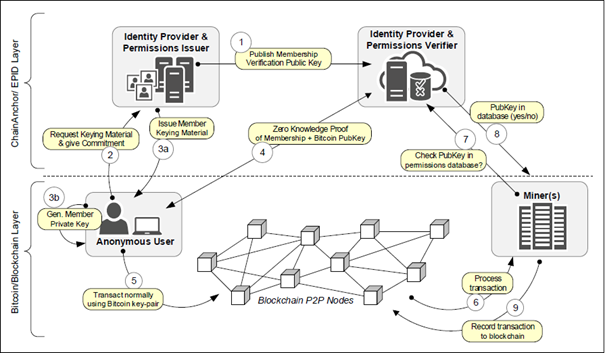
\includegraphics{anonymous_identities_for_permissioned_blockchains.png}

Privacy is established by spreading the non anonymous interaction of the user across multiple organizational entities, so that each entity only has access to a small part of the users non masked identity.\cite[p.4-5]{hardjono2016anonymous}
\begin{itemize}
\item \textbf{Permission Issuer:}
Knows each given users personal key pairs, but has no knowledge of their bitcoin keys.
\item \textbf{Permission Verifier:}
Knows each given user's membership key pairs and transactional key pairs, but has no knowledge of their personal key pairs used in obtaining group membership key pairs. However each user part of the same group will look the same to the verifier
\item \textbf{Additional Privacy:}
User is able to choose his own permission verification entity, so that the risk of collusion between parties is reduced immensely
\end{itemize}

\subsection{Assumptions about the underlying System}
\begin{itemize}
\item Permission issuer and permission verifier are separate entities and not in collusion (physically, operationally, legally separate entities)\cite[p.4]{hardjono2016anonymous}
\item User has Trusted Platform Module\cite[p.2-3]{hardjono2016anonymous}
\item Single permission issuer, however multiple permission verifier\cite[p.5]{hardjono2016anonymous}
\item During setup it is assumed that the permission issuer has a secure channel with mutual authentication to the permission verifier for transference of the membership verification public key\cite[p.5]{hardjono2016anonymous}
\item During user registration for permissioned groups it is assumed that the user and the permission issuer have a secure channel with mutual authentication\cite[p.6]{hardjono2016anonymous}
\end{itemize}

\subsection{Continuing Work}
In the coming months the authors are going to focus on supporting anonymous attribute groups in identity providers. These are called assertions in SAML2.0 or claims in OpenID-Connect and verification is obtained from external sources or attribute authorities. Furthermore they are working on implementing a RESTful design for their zero-knowledge proof protocol and support for Anti-Money Laundering (AML).\cite[p.17]{hardjono2016anonymous}



\chapter{Concept and Design}
\label{cha:conceptanddesign}

\section{General}

\section{Requirements and Challenges}

\subsection{Requirements}

\subsubsection{GDPR compliance}
The General Data Protection Regulation (GDPR) is a regulation by the European Parliament, Council of the European Union and the European Commission focused on strengthening EU citizens digital privacy.  Its main focus is on giving citizens control over their digital personal information and simplifying the regulatory environment for multinational corporations. However it also adds a strict data compliance regime, by penalizing transgressions with up to 4\% worldwide turnover\cite{gdpr}. Furthermore this regulation does not have to be verified by each EU's regulatory body, since it is a EU regulation, compared to an EU directive which has to be ratified by each EU signatory state.

\section{Challenges}
\label{sec:challenges}

\subsection{Security Goals}
\label{sec:securityGoals}

Designing a identity management systems comes with various legal implications. We are referring here to § 9 “Technical and organizational actions” in the “Federal Data Protection Act”\footnote{Translated from the German language “Bundesdatenschutzgesetz”} were an identity management system shell enforce all necessary measures to protect identity information.\cite{bdsg}

So we will focus on the following security goals:
\begin{enumerate}
\item \textbf{Confidentiality:} Data shell be secured on its transmission. This includes the blockchain and communication over the internet. 
\item \textbf{Integrity:} The integrity of the data needs to be assured so that no entity can change identity information without knowledge. 
\item \textbf{Authenticity:} Identity information are protected against unauthorized access. 
\item \textbf{Non-Repudiation:} No entity can deny having taken an action.
\item \textbf{Privacy:} The privacy of a user is preserved while interacting with the system. 
\end{enumerate}

We further also see the blockchain as a world open readable ledger were everyone can read transactions or information stored on the blockchain. So interactions with the blockchain need to ensure to not expose any identity information. 
It is not allowed to store hashes or encryption of claim in the blockchain, since it is a tamper-proof data storage, information can not be removed once written. So if the hash or encryption gets broken the identity information is leaked and can not be removed.  

\subsection{User Acceptance}
\label{sec:userAcceptance}

TODO Oskar
Switching from offline to online identity is an unspecified burden that falls into the eye of a common pleb.
Especially for elderly and uneducated the imagination of not having a piece of paper with an id and not having a central
institution that takes care of one's identity is suspect, if not horrifying.
Not only the lack of a trusted party but also the concept of blockchain, smart contracts and all of its gists are unknown
to most people. This leads to further distrust in the system.

By introducing such system, a lot of clarification for non-technical people and common folks therefore needs to have a
high priority.

Without understanding the process and system, users run the risk of being exploited and not being aware of what information
they are currently sharing.

\subsection{Economic feasibility}
\label{sec:economicFeasibility}
In order for a new system to become succesful, it is imperative that it is econimically feasible. Its total cost of ownership should be comparable to or even lower than the system it is replacing.
However the total cost of ownership of an identity system where the blockchain is used for storing transactional information is extremely difficult to gauge. This is in part because it is a "living platform" which is constantly being changed, but also because of the volatility of cryptocurrencies.\cite{elendner2016cross}
Due to cryptos nature it is difficult to keep costs stable or predictable, since accurate models are still actively being worked on.\cite{catania2018predicting} The slightest change in financial regulation, bad press, or just negative comments in social media can crash their prices.\cite{kim2016predicting}
In contrast their prices can also rise in an astonishing fashion because of aforementioned reasons. 

This projects aim however has not been to create an economically feasible platform, but a simple demonstrator, showcasing that blockchain technologies could be adapted to suit the societal needs of a digitalized society. \projectName{} can be used as a digital alternative to an already existing non-digital system.
However before a full deployment could take place further development is necessary to minimize all costs associated with the interactions with the blockchain.

As an alternative solution however it would be possible to replace the public blockchain with a governmentally run private network. This would reduce the costs of transactions by giving the owning entity full control over all costs associated with the blockchain transactions.
This however would also cancel the independent miners motivation to be part of the system. Creating the need for different remuneration concepts or even state owned miners. These proposals however would introduce new risks into the system by defining a single trust anchor for the entire system. 

\section{Processes}

\subsection{Registration}
In order to be part of our distributed digital identity system that we envisioned, it is necessary to register with it first. The registration process consists of the following steps (See Figure \ref{fig:registration_concept}):

\begin{enumerate}
\item \label{registrar_item_one}
The user creates an ethereum address and a private public key pair, the combination of these two are now used as the users digital identity. Jointly they can be used as a digital identity card. They are safely and securely stored in the users own database.
\item \label{registrar_item_two}
For verification and auditing purposes these have to be verified by a trusted party, so that third parties can be sure of the identity of the individuals. We are using a specially designed smart contract, where the user inputs his ethereum address and his public key. Once filled, he writes it to the blockchain and waits for the trusted party, in our case a governmental agency, to check the contents, fulfill and sign the contract.
\item \label{registrar_item_three}
The user now verifies himself using the eID online verification system. After successfully verifying he sends the governmental agency, entrusted with handling digital identity services, his ethereum address and public key. These are used for the upcoming smart contract verification.
\begin{comment}
DONT NEED: The user can now have his ethereum address and private public key pair verified by a governmental agency.
\end{comment}
\item \label{registrar_item_four}
The aforementioned governmental agency can now check the blockchain for the requesting users registrar contract, verify its content against already received (See \ref{registrar_item_three}) or saved information and then link the existing user to the ethereum address and public key. After extending the database entry the agency now collects all existing claims for that individual, packages them into a single claims object and sends it to the user for his record keeping and claim query construction.  
\item \label{registrar_item_five}
Lastly the agency signs and approves this registrar contract. By adding its signature the user is now a fully registered member within our community. Henceforth he can use this identity to request services and offer claims to and from other registered parties. 
\end{enumerate}

\begin{figure}[ht]
\centering
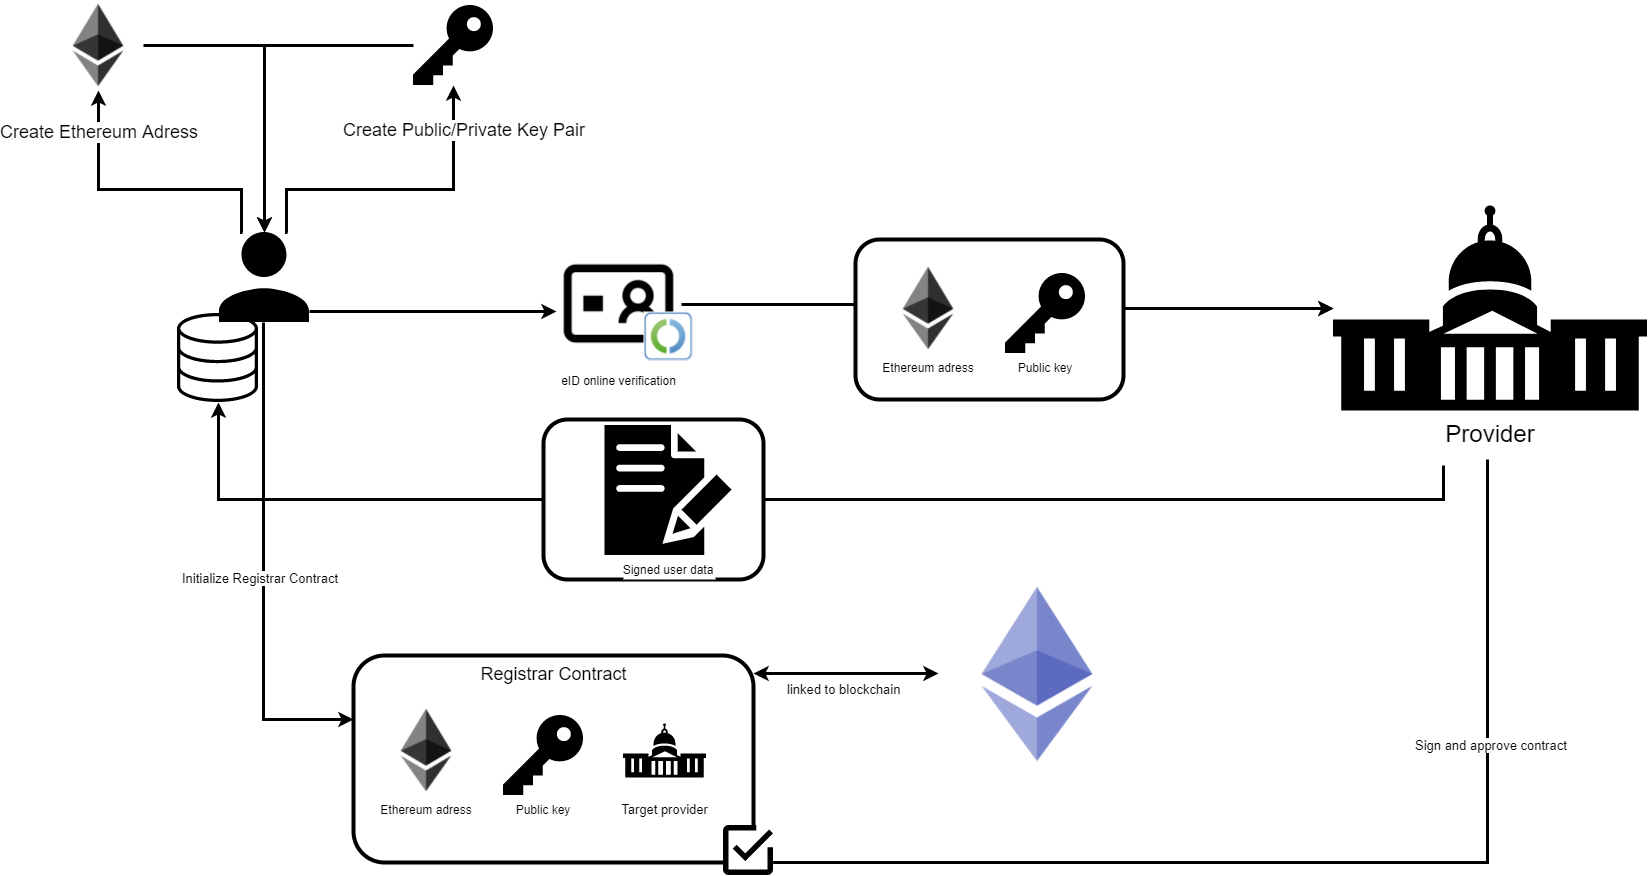
\includegraphics[width=\textwidth]{concept/registration.png}
\caption{Registration}
\label{fig:registration_concept}
\end{figure}

\subsection{Permission Request}
Permission requests are an integral part of our system. They are the 


After registration the user is now able to use \projectName{} for identification and verification purposes. Lets consider opening a new bank account using \projectName() for verification.

% Please agument why the user if he is holding signed claims is not providing his claims directly to the requesting provider
% Include the following arguments:
% 1. request shell be populated through the blockchain so that every entity can acknowledge the claim sharing
% 2. populatring thre reuqest through the blockchain gives us the possibility to explicit approve the sharing
% 3. generating a signed query can also have additional attributes like a reuse flag to indicate if the query could be used again if the claim changed
% 4. user don't have to pay for the creation of the smart contract. only for the updating of the signed values

\begin{enumerate}
\item \label{permission_request_item_one}
We have a user called Tom who has just recently moved and is interested in opening a new bank account for his local dealings. He therefore visits a local branch of Bank X and requests a new bank account. He now hands his ethereum address, public key, Name, Address etc. to the bank teller.
\item \label{permission_request_item_two}
The bank teller now enters that information into a \textbf{Request Permission} form and sends it to the government for verification purposes.
\item \label{permission_request_item_three}
The government now writes a new permission request contract into the Ethereum blockchain. This contract contains the following information:
\begin{itemize}
\item @EthereumAddress; This is Toms Address, as his information is requested
\item ThirdPartyName; This is the requesting Party's Name Bank 
\item AttributesRequested[GivenName, FamilyName, StreetName, StreetNumber, PostalCode, DateOfBirth, ...]; This is an Array containing all Variables requested by the Third Party
\end{itemize}
\item \label{permission_request_item_four}
The user now polls the blockchain for new messages and finds this permission request by the third party.
\item \label{permission_request_item_five}
Tom now checks each requested attribute and selects the attributes he wants to share with the third party. After his selection a specific query is created imitating his choices.
\end{enumerate}

\begin{figure}[ht]
\centering
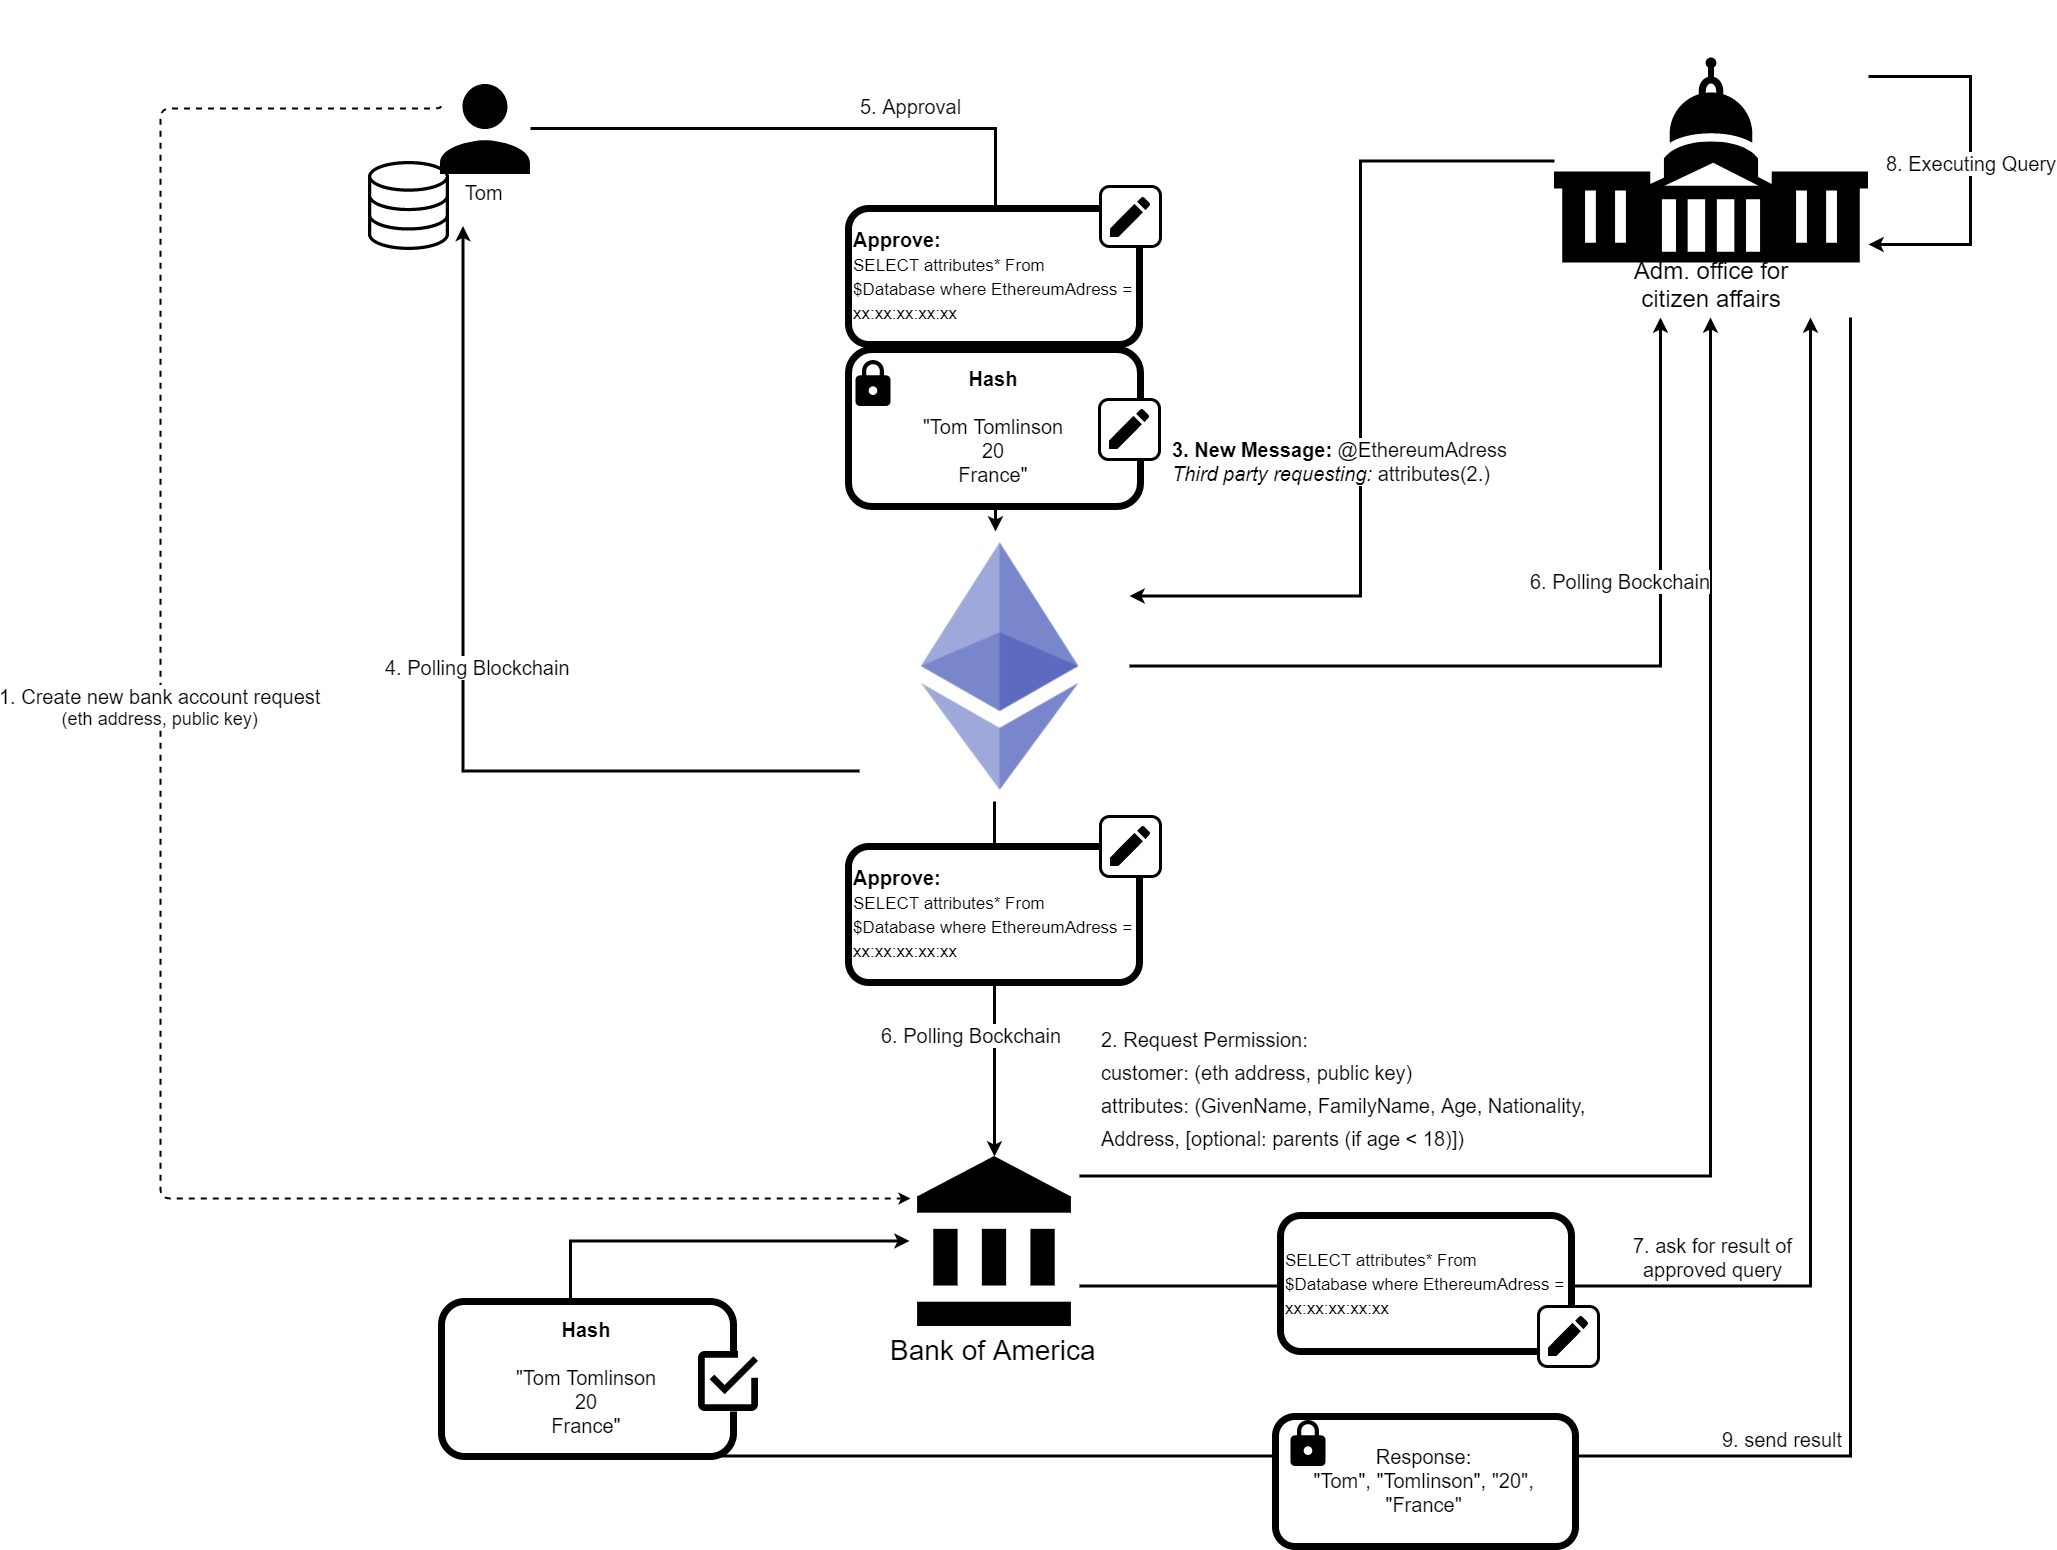
\includegraphics[width=\textwidth]{concept/permission_request_bank.png}
\caption{Permission Request}
\label{fig:permission_request}
\end{figure}

\subsection{Closures}
%Create closure figure in draw.io and insert here
\begin{comment}
\begin{figure}[ht]
\centering
\includegraphics[width=\textwidth]{concept/closure.png}
\caption{Closure}
\label{fig:closure}
\end{figure}
\end{comment}

\subsection{Changing Claims}

\begin{figure}
 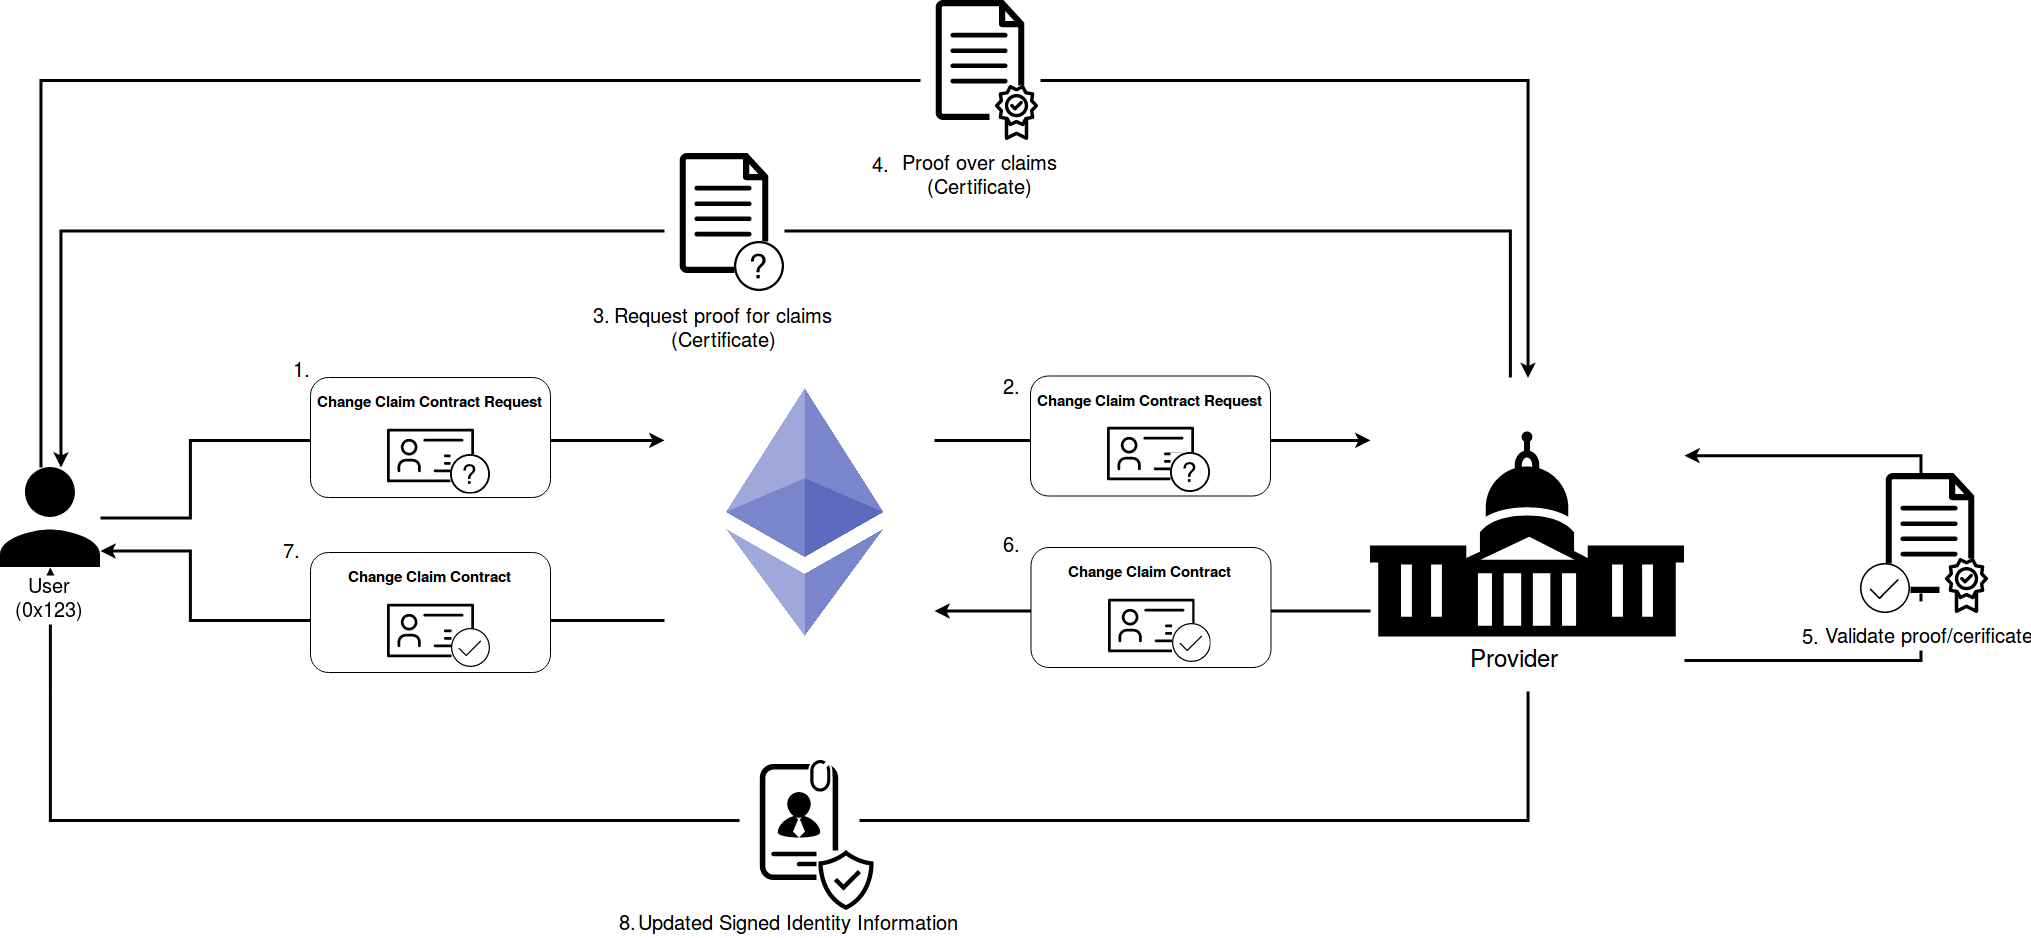
\includegraphics[width=\textwidth]{concept/change_claim.png}
 \centering
\caption{Concept of the change claim work flow. Change claim events are populated trough the blockchain so that every provider holding the same claim for the referenced user can start a new permission request to update the claim values.}
\label{fig:changeClaimsFig}
\end{figure}

Changing claims in a self-sovereign manner with still providing the high level of trust in this claims is a challenge. We evaluated two entry points for this contract: a) the user starts the procedure by sending a “change claim contract request” or b) the government enforces new claims by populating a “change claim contract”. 

Both actions are described as use cases in section \ref{sec:changeClaimUseCase}. For a) the use case that the user may want to change his family name because he got married recently. In the case of b) the government triggers a change claim as an law enforcement (e.g. the user looses his driving license for a certain time) or an other federal institution wants to update the users claims. Each scenarios are described in detail in this section. 

To still serve as a self-sovereign system the user gets the possibility to create a “change claim contract request” (step 1., figure \ref{fig:changeClaimsFig}). This contract itself does not enforce any change of any attributes, but serves as a change claim application. The user states the claim IDs he wants to change inside the contract. He may even add additional attributes like a time period to define for how long the claim shell be changed. It is also possible to propose new claims the user want to add by himself. However, new or changed claims needs to be verifiable by the provider. The “change claim contract request” is likely addressed at the institution that would have the highest trust level in the system, since the signature over this claims is only trusted as much as the institution itself. In our scenario the government satisfies this trust level. Some might argue that it is not necessary to populate the “change claim contract request” trough the blockchain (since each transaction cost money), but it helps to establish more transparency in our system and relocates power to the user. He decides which claims he wants to change and which new claims he wants to have added to his digital identity. 

The government pulls down the “change claim contract request” and evaluates, it in step 2., for which claims it needs a verification, e.g. a certificate. Off-blockchain the user is asked for a proof or certificate over his proposed claims (step 3.). Each provider can define which kind of proof the user must provide to get his claim changed. The level of trust in a provider grows with the amount of accuracy the provider puts in his claim validation. The user provides the proof in step 4. Since different provider may accept different proofs, it can be various documents, like photos of his ID card, certificates of his club membership or even audio recordings. However, if the user is not able to provide the necessary proofs, the contract will be killed and the change claim request rejected.
The provider validates if the provided proofs satisfies his acceptance criteria in step 5.  If the proofs are sufficient the provider accepts the “Change claim contract request” by setting a flag in the contract, or even removing some claims from the contract on which the verification failed (step 6.). 

Now every other provider in the system holding old claim values for the referenced user can create a new permission request to discover the new changed claims from the provider handling the change claim contract. The user still needs to approve the new incoming permission requests. In step 7. the user gets the notification about the successful approval of the change claim contract and queries the provider to retrieve a signed version of his updated claims (step 8.). 

Here the change claim process is finished. However, as mentioned previous there is also a scenario where a federal institution wants to enforce a claim change (for example the temporary removal of driving license). In that case we would directly start at step 6. where the government will publish an already approved “change claim contract” referring to the claim IDs that were changed and additional values restricting the duration of this enforcement. Extern observers of the blockchain will notice that it is an enforced claim change since the user did not provide a “change claim contract request”. In the same way as described previously, the provider will take note about the claim change and can setup a new permission request to discover the new claims. As a side note: If the user rejects the permission requests the providers holding outdated claim values can simply distrust this values and decide if they are still  willing to provide the user service with outdated values. Please referrer to section \ref{sec:changeClaimUseCase} for a use case.

\subsection{Evaluation}

 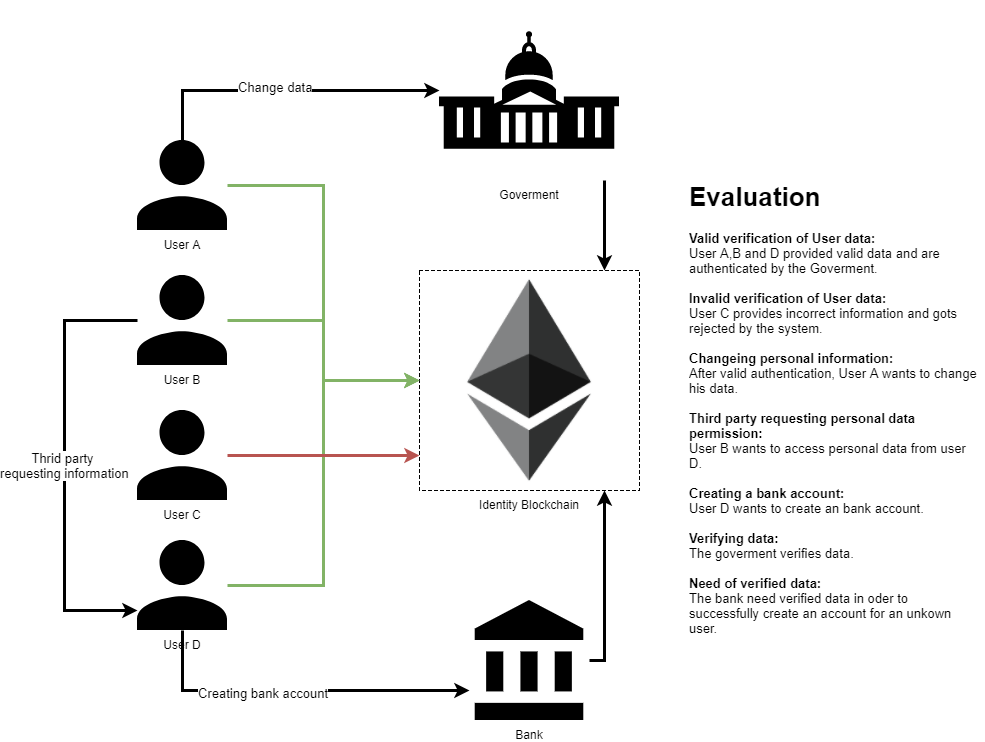
\includegraphics[width=\textwidth]{concept/evaluation.png}
 
\section{Use cases}

\subsection{Change a claim}
\label{sec:changeClaimUseCase}
\textbf{a) User changes claims:}
Lets have a user Bob Bobsen who has recently married Alice Alicson. Since Bob wants to change his family name to Bob Alicon this information needs to be updated in our system. To do so he creates a new “Change Claim Contract Request” holding the “FAMILY\_NAME” claim ID and addressing this contract to the government. The government will ask Bob for his marriage certificate. Bob sends his certificate over a secured connection to the government. They, on the other hand, can now verify the new claim by checking Bob's marriage contract. If the certificate is authentic the identity provider publishes an approve transaction to the change claim contract to notify all third parties and other identity providers about the new claim of Bob's digital identity.
Bob does then pull the blockchain, and requests the signed version of his new family name from the government, which he saves in his local database.

\textbf{b) Enforced claim changes:}
Bob has lost his driving license by a moderate traffic crime. Since Bob is still holding a signed version of his driving license in his local database he could easy rend a new car. So the government enforces a claim change by publishing a “Change Claim Contract” to the blockchain referencing Bobs ethereum ID, the driving license claim ID and a time period (6 month). Each entity observing the blockchain can within his 6 month distrust the driving license claim value provided by Bob, if the provided signature is older then the creation date of the “Change Claim Contract”. However, Bob can query the government for the updated claim value and retrieve the temporary restricted driving license, which is then also trusted, because it is up to date. After 6 month no new claim change contract needs to be setup because an entity can simply compute that the restriction time is expired and that no new claim change was published by the government. 

\chapter{Implementation}
\label{cha:implementation}

\section{Core-Logic}
Blockchain-Identity is always focus around two actors: The user and his interaction with the blockchain and identity providers and their interaction with the user in an on- and off-blockchain fashion. We model our system in the same way but needed to make some specifications for the provider service which comes with two different motivations and rights:

\begin{itemize}
\item \textbf{Normal Provider}: Holds domain specific personal data about their consumers that are not exposed to the outside world. They have an interest in requesting user data to extend their system and to make new costumer registration easier. This services are untrusted and can not write to the blockchain. However they can read from the blockchain to verify transactions or extract information out of it. In general everyone can setup a provider service and request user data. They don’t need to be verified in any kind. 
\item \textbf{Government}: Single trusted entity that holds verifiable citizen information. This information are backed by the representative citizen office or other federal trusted institutions. The government usually verifies user data.
The government service is the only service that can read and write to the blockchain. 

The client application, on the other hand, has read and write rights and can interact with this providers.

This following sections descriptes the different provider/client applications and their interactions with the other components: frontend, Etherem-Blockchain-Adapter – EBA and the database.
\end{itemize}

\subsection{Motivation}
Since we are dealing with provider which are providing user information data we decided to implement a normal client-server architecture. Here we can use all the advantages TCP is providing us like transport layer encryption with SSL/TLS and the reliability/inorder-delivery TCP comes with. Where we would have to deal with our own encrypt-scheme if we would use UDP with peer-to-peer communication and port discovery, even if peer-to-peer communication seems like the more fitting solution since we are already in the domain of blockchain and decentralized applications. 

Choosing a client-server architecture comes with the drawback that the government service can not notify the client about incoming messages. The communication via the blockchain is not possible since the provider have not permission to write to it. To overcome this challenge we implemented a discovery service where each components registers to on bootstrap. (See section \ref{sec:discoveryService}).

We further decided to design our services RESTful (Representational state transfer). This in mind spring boot\footnote{\url{https://projects.spring.io/spring-boot/}} is a good choice in the Java domain for rapid prototyping. Spring boot also offers good integration for database adapters and spring security\footnote{\url{https://projects.spring.io/spring-security/}} a authentication and authorization framework. 

\subsubsection{Tools and Technologies}
Besides Sprint Boot and Spring Security we further committed us to the following technology stack: 

\begin{itemize}
\item Springfox\footnote{\url{https://springfox.github.io/springfox/}}: A API documentation framework. Additionally is is specifically designed for spring boot.
\item Feigen\footnote{\url{https://github.com/OpenFeign/feign}}: Framework that make writing API calls easier. You only need to provide an interface and specify it with annotations to produce a HTTP request to specific domain. Mapping and error handling is mostly done by Feigen. 
\item Lombok\footnote{\url{https://projectlombok.org/}}: Lombok reduces the boilerplate code in Java by directly translating data or logging annotation into java byte code. It helps us to reduce the size of our models to a minimum by obscuring the setter, getter and constructors. 
\item Bouncy Castle\footnote{\url{https://www.bouncycastle.org/java.html}}: The unofficial default cryptographic library for java. It implements the java security provider interface and provides a functions like RSA encryption or signature mechanism.
\item Zxing\footnote{\url{https://github.com/zxing/zxing}}: Library to generate QR- and bar-codes. 
\item Web3j\footnote{\url{https://web3j.io/}}: Library providing the Ethereum adapter. (More in section \ref{section:eba}. In this section this library is mainly used to generate ECDSA (Elliptic Curve with Digital Signature Algorithm) signatures. 
\end{itemize}

Further the following technologies are used for testing:

\begin{itemize}
\item AssertJ\footnote{\url{https://joel-costigliola.github.io/assertj/}}: A fluent assertion semantic for java. 
\item Mockito\footnote{\url{http://site.mockito.org/}}: Mocking library to make unit and rest test more modular and encapsulated from outstanding components. 
\end{itemize}

\subsection{Components}
\begin{figure}
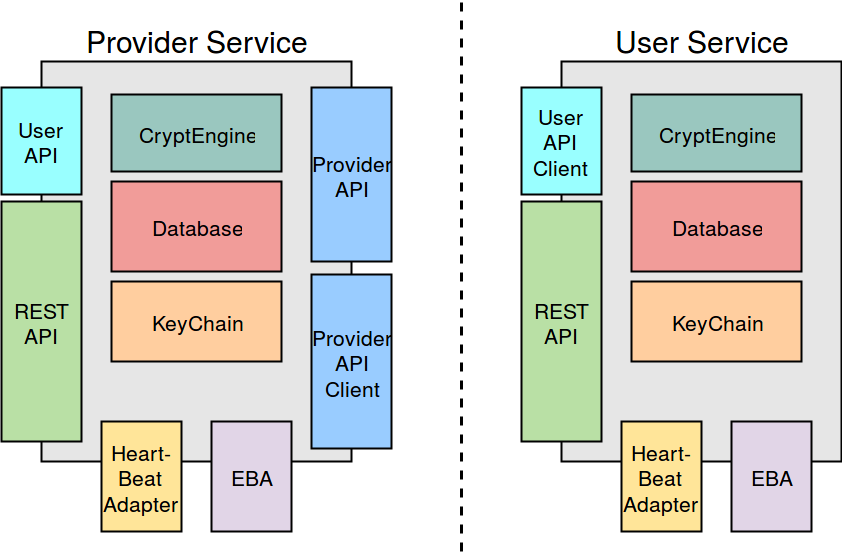
\includegraphics[width=0.7\textwidth]{impl/ComponentDiagram.png}
\centering
\caption{Overview about the components of an individual service and their exposed endpoints. Left is the provider service providing also a provider API and provider API client. Right the user service implementing the client API client.}
\label{fig:componentDiagram}
\end{figure}

In figure \ref{fig:componentDiagram} you can see an overview about the components in the provider and user service. All boxes that are drown over the border are representations of exposed endpoints or clients and inside the box are the core components listed.

\subsubsection{Internal components}
The crypt engine is the main framework for encrypting, decrypting, signing, validating signatures and generating hashes. It provides methods for symmetric and asymmetric encryption. It uses bouncy castles as security provider to generate keys and handle cryptography. To generate elliptic curve signatures it uses the framework provided by web3j. 

We are using spring data to provide a very easy interface to couchbase, our database storage (section \ref{sec:database}). The keychain is the current session object holding the RSA key-pair, EC key-pair and some other meta information about the current state of the service. This objects gets cleared if the services logs out and restored if the service logs in (section \ref{sec:registerContract}). 

\subsubsection{User API}
\label{sec:userAPI}
The user api provided by a provider service and requested by the user service defines the central entry point of client requests to a provider. The user and the provider API (section \ref{sec:providerAPI} is implemented as a normal Java interface. The provider service is implementing this interface and mapping the defined methods to REST endpoints which then are bounded to a predefined paths. The user service on the other hand, extends this interface in a new interface which then serves as a Feign adapter bound to the same predefined paths. This is really convenient because Feign needs an annotated interface to build an REST client out if it. We only have to bind Feign to the same resources paths the provider is exposing so that they can communicate to each other. 

\subsubsection{Provider API}
\label{sec:providerAPI}
The provider API is a unified interface which each provider is offering in form of REST endpoints. Each provider builds also a Feign client (see section \ref{sec:userAPI}) to talk to other providers.  Via this API provider an interact with each other to exchange requests or offering services. Notably is that each request needs to be authenticated via a SignedRequest (see section \ref{sec:ecdsa}) to ensure that only authenticated entities request this API. 

\subsubsection{REST API}
The rest API is the connection to the frontend. Here the frontend can ask for user resources and claims to display them a web admin or the end user. This requests are backed by a basic authentication mechanism which is not optimal because the password and user name is transmitted in plain text if no transport layer encryption is used. The plan was to change this mechanism since to a more secure scheme like Json-Web-Token (JWT) authentication, but that would require changes in other components and was also out of scope of the core focus of this project. 

\subsubsection{HeartBeatAdapter and EBA}
Ethereum Blockchain Adapter (EBA) is the entry point to communicate with the blockchain. We defined an interface (EBAInterface) between the blockchain component and the core-logic to develop in a parallel fashion. Relate to the section \ref{sec:eba} where everything related to the blockchain is explained.

The HeartBeatAdapter is the connection to the Discovery Service (section \ref{sec:discoveryService}). A service can register itself to the discovery service, create or subscribe to new beats.

\subsection{Notable methods}
The follow sections describe problem and challenges that occurred during development.

\subsubsection{Serializing and deserialization of arbitrary objects}
\label{sec:serialobject}

Serialization of arbitrary objects is a challenge in systems where the order of serialization is imported (e.g. building a signature via hashing over the serialization outcome). A common serialization method is the JSON-String serialization, where an arbitrary object state gets converted into a JSON representation. This can be done by (for example) the Jackson object mapper\footnote{\url{https://github.com/FasterXML/jackson}}. We need, however, define the order  in which each field of the object gets serialized. Serializing all objects into JSON representation allows us to serialize the objects in the same way all the time, no matter if it is a signed request against the blockchain or a response to the frontend. 

The other approach is to use Javas serialization API. Classes that implement "Serializable" will then be converted to a stream which then can be collected to a byte array. Since Java serialization will take care of the serialization order by itself we don’t have to bother with that. 

However, we need to find a unique way to serialize objects since building a hash-based signature via objects must be done always in the same way, no matter on which system the signing or verification of the signature is happening. We decided to use JSON serialization approach (with explicitly defining the order in which properties shell be serialized) since it is language independent, easier to implement and to debug, even if it is not as efficient as raw byte representation. How signatures are build and verified is described in the next section \ref{sec:ecdsa}. 

The implementation of sets in the Java Virtual Machine needed also consideration. Sets are of nature unordered and it depends on the order of object initialization on the heap to define the real order the elements returned in. If you want the same order of object each time, you need to use lists. Building a hash over an object holding sets is obviously a bad idea since the order of attributes may be different from machine to machine, so the hash will be a different.  

Another problem related to serialization was that variables of type "Object" will be converted into a string representation and on deseralization this string will not be converted back in the original type since "String" itself extends "Object". This became a problem on serialization of LocalDateTime values, which were not parsed back into a LocalDateTime. 

To temporary handle the different conversions we implemented a "ValueHolder", a simple class separating LocalDateTime values from generic Object values. By converting explicit into a LocalDateTime the Jackson converter recognizes the string representation and deserialize it into the correct object representation. Future improvements can be made by including the target class of the serialized value as meta information, so that in deseralization the value can be parsed back to its original class. Further the object mapper need to be adapted adequately. 

\subsubsection{ECDSA and SignedRequests}
\label{sec:ecdsa}

Elliptic Curve Digital Signature Algorithm (ECDSA) in the SECP256k1 configuration is used by Bitcoin and Ethereum to sign transaction to the blockchain. \cite{mayer2016ecdsa} This ensures integrity and authenticity to the sender and the content of the transaction. 

To populate this security properties also between services we use ECDSA also for inter service communication. This is done by generating a so called "signedRequest". This object can hold a generic payload and the EC Digital-Signature over this payload. This payload but needs to include the ethereum address of the sender (similar to ethereum transactions). A signature is then build in the following way: 

\begin{enumerate}
\item The payload (holding also the ethereum address of the signer) gets converted to a JSON as defined in section \ref{sec:serialobject}
\item A SHA-256 hash is build over the given JSON
\item This hash will then be signed by the ECDSA and the private key (EC) of the signer
\item The resulting signature gets appended in the signed request for validation
\end{enumerate}

\noindent The validator on the other hand can validate the signature by applying the following steps:

\begin{enumerate}
\item Convert the payload to a JSON with the same object mapper configuration as used for serialization.
\item Create a SHA-256 hash itself over the generated JSON
\item Validate the provided signature against the computed hash. Interesting to know is that his validation does not yield a boolean flag but a computed ethereum address the algorithm "thinks" that signed the request. 
\item We take this generated ethereum address to check it against the included ethereum address in the payload. If they are equal yield true, else false. 
\end{enumerate}

If we would not have include the ethereum address of the sender inside the signed payload an malicious attacker may have exchanged it against a valid signature address. 
To validate and build signatures over Java objects we are using the Jackson object mapper module \lstinline{jackson-datatype-jsr310} in version \lstinline{2.8.10}. This module is further configuration to write time values as a time stamp in the ISO-8601 format. 

\subsection{Discovery Service}
\label{sec:discoveryService}
As mentioned in the previous section the Discovery Service is the result of a client-server architecture in a peer-to-peer environment. But it further serves additional purpose for holding and distributing RSA public keys, discovering domain names, where to find the exposed API and if the requested service is online. 

While all the stored information is public visible no sensitive data is exposed in the Discovery Service. It just provides connection information and serves as a message broker. Each stored entry needs to be signed by the author with the private key bound to his ethereum address. All unauthorized requests are rejected by the service. By ensuring the authenticity of each entry creation or update it is ensured that no service spoofing can happen. Only the holder of the private key bound to his ethereum address can update his connection information.

\subsubsection{Beats}
\label{sec:beats}
Beats are the messages that are routed by the Discovery Service. A \textit{beat} a small package containing an event type describing that kind of message it is and a subject field referencing the location where the new information is to find. Each beat is uniquely identified by the combination of recipient ethereum address and the current beat number (incrementing per beat). 

There are two types of subjects: The URL references a API endpoint where new or updates information are now present. The recipient is requested to request this API endpoint to update his information state. The other kind of subject is a ethereum address: The recipient is requested to query the blockchain for the given address to process the information stored at this address. 

On registration entities start to periodically (each 10 seconds) ping the Discovery Service to wait for new incoming beats. Since the discovery service itself is not a trusted entity, each beat gets verified before processing and it is checked that the signature matches the senders ethereum address.

\subsubsection{PKI}
\label{sec:pki}

A Public-Key-Infrastructure (PKI) is an infrastructure to bound identities to public keys. This usually relay on trust in either a Certificate Authority or on other users trusting this public key. 

Since each entity stores also his RSA public key into the discovery service and sign this entry with his EC private key, the trust of the given RSA public key is tightly bound this EC key pair. If the RSA key gets stolen it can be simply replaced in the Discovery Service. If the EC key gets stolen both key pairs need to be regenerated. How we establish trust in the EC key pair is explained in the next section.

\subsection{Register Contract}
\label{sec:registerContract}
\begin{figure}
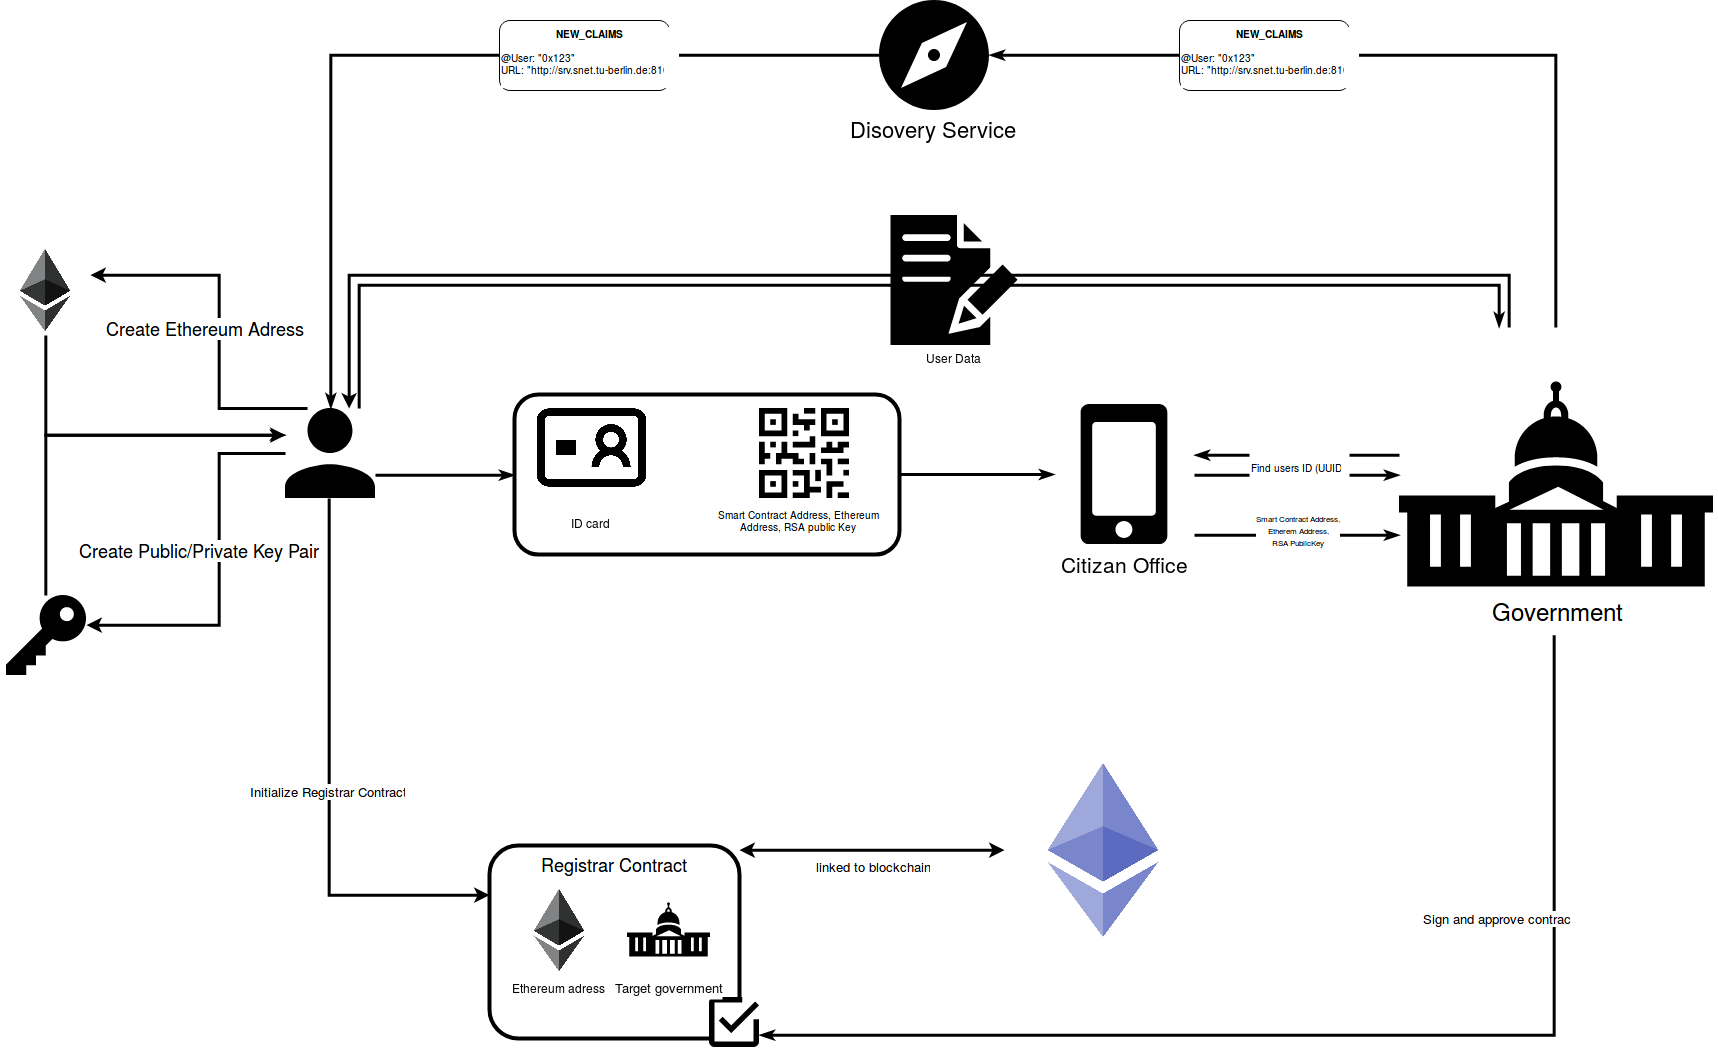
\includegraphics[width=\textwidth]{impl/RegisterContractImpl.png}
\centering
\caption{Implementation of the Register Contract flow. Since it was not possible (time limitations) to include the eID verification mechanism, we implemented the in-person verification. Here the newly register user has to go the citizen office to how his ID card to gets his ethereum address, RSA public key and smart contract address verified.}
\label{fig:registerContractImpl}
\end{figure}

To start the register process the user services exposes the unsecured resources "Account" which provides action endpoints for login, logout, register and QR-code retrieval (later more on that), where the web client can make a HTTP-POST call to "account/register" with a newly set password.
This call will trigger three main actions:

\begin{enumerate}
\item Creating a 4096-bit security RSA key pair
\item Creating a new wallet containing EC-Key Pair 
\item Setting up the register contract 
\end{enumerate}

\subsubsection{Creating RSA and EC key pairs}
We need the RSA key-pair to later encrypt sensitive data that is send via the blockchain since the blockchain itself is a public ledger and for everyone readable. The key-pair created by web3j does not provide any confidentiality since the ECDSA (Elliptic Curve Digital Signature Algorithm) can only be used to generate and verify signatures (see section \ref{sec:ecdsa}). So the users creates a 4096-bit strong RSA key pair (step 1.1). So ensure that this key indeed belongs to the newly generated EC key-pair (step 1.2) we generate a signature, as mentioned previously (section \ref{sec:pki}), over the RSA public key with the EC private key and publish this information to the discovery service.

We further also save our keys, password based symmetric encrypted, to our data directory under \lstinline|{$USER.HOME}./ethereum/blockchain-identity/|\footnote{The "./ethereum" directory is the default directory to save all ethereum related files.}. If the user later logs out, we can simply remove the current RSA and EC keys from memory and if the user logs in again, providing his password, we can decrypt the wallet files and read the RSA and EC keys back in memory. 

The user service application is planned to run locally on the users host machine. This would secure it from outside access. Since we, because of time limitations, didn’t manage to implement a key recovery mechanism there might be an Denial-of-Service attack vector possible where a malicious application running also locally on the users host machine, call periodically the register-endpoint, preventing the user from accessing his information because his keys gets reshuffled every time. Some could think about disabling this register endpoint after successful creating a key pair, but since this is a prototype under developing this endpoint needs to be open and accessible. 

\subsubsection{Deploying the register contract}
The ethereum address itself is a just a representation of the EC public key. To now register the user that is bound to his ethereum address we setup a register contract (step 2.). This register contract is just a public representation of the unverified user and contains no more information then the users ethereum address and a flag if the user is approved. This flag can only be set by the trusted government. 

\subsubsection{Verifying the user}
As shown in figure \ref{fig:registerContractImpl} the user then creates a QR-Code (step 3.) to encode his ethereum address, address of the smart contract and his public key into it.\footnote{It is not necessary to encode the public key into the QR-code at all since the Discovery Service also stores this information, but we can save an additional request from the government side to discover it by providing it in the register flow directly.} The QR-code generation is done with the help of the Xzing library and exposed via an rest endpoint "/account/qr-code". The idea to generate a QR-code is simply that ethereum addresses are quite hard to type and since the user has to go to the citizen office in person he might as well just show is representative QR-code. 

The citizen office verifies that the user is indeed who he claims to be with the use of the provided ID card. The android application build for the purpose of scanning the QR-code, generating a signature over the retrieved information and sending it to the government service, needs further know which user is currently trying to be verified to the system. To do so the citizen office types in the user information found on the ID card, for example given name, family name, etc. to then send a authorized requests to the government which then queries its database for a user with the same information and returns his UUID (step 4.). 

With the retrieved UUID the application can then make a signed POST request to the user resource that tries to get verified and updates the user for his public key, ethereum address and register contract address (step 5.).

\subsubsection{Finalize user registration}
The government then uses the information about the user to update the register contract to set the approval flag to true (step 6.). So that every party in the system observing the blockchain can verify that the user holding the private key for the ethereum address is indeed verified by the government. If each provider checks that he is only communicating with verified users we are preventing sibyl attacks in the most effective way possible. There would be no need to use CAPTURES since only verified users are able to interact with the system. 

It also creates a new signed beat (section \ref{sec:beats}, step 7.1 and 7.2) with the information "NEW\_CLAIMS" addressed at the users ethereum address to notify the user to request its provider API (section \ref{sec:providerAPI} to retrieve the claims stored at the government about him (step 8.). 

Since a new user is now verified in the system other provider shell also send the user their claims about him. That point was really difficult to implement and was left open for further work since there are open unanswered questions: How do provider assign the new ethereum address of the newly registered user to any user of their system (you can not broadcast any user claims over the network because of privacy reasons)? How to ensure that provider send all their claims (since they are not trusted they might be malicious)? 
In the end we said that the user has to manually notify provider about his presents in the system.

\chapter{Evaluation}
\label{cha:evaluation}

\projectName{} is a prototype implementation of a GDPR complaint solution of self-sovereign identity management in the blockchain. Since this project is more a proof-of-concept then a working platform, we will do a critical review of the implementation and concept section and outline the building blocks for future work.  

\section{Core-Logic}
\label{sec:coreLogicEval}
Since the whole system is a prototype there are several improvements and alternative design choices that could increase security and stability in the proposed system.

\subsection{Decentralized untrusted system}
\label{sec:untrustedSystem}
If we drop the principle of a private blockchain and let every provider write to the blockchain as well, we deescalate the government as single point of failure. To ensure further availability we could drop the discovery service and organize the discovery of an specific provider in a distributed hash table. Since we want still off-blockchain communication we could think about a peer-to-peer implementation which will completely decentralize the system. The final problem that still remains is how to establish trust in a new user without having the government as a trusted party? Since we already considered the eID of the German government as a verification mechanism we can take this to the next level by allowing the peers to retrieve identity information from the eID directly. By doing so we would finally eliminate the government as needed, trusted party and can relay only heavily on the trust already established in the certificate which signed eID of the user\footnote{Of cause this certificate is still generated by the government but the government as such would be eliminated as central component where requests would be routed though.}.

\begin{figure}
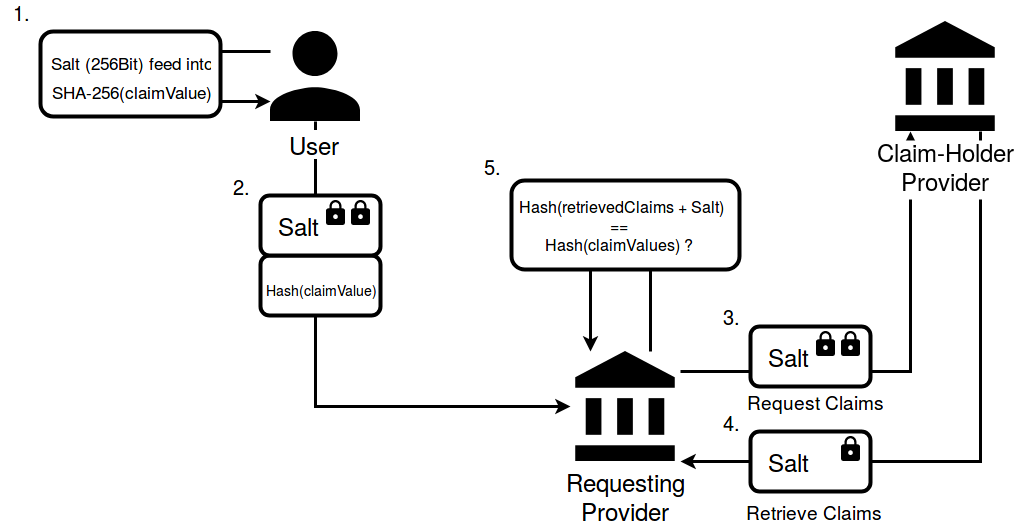
\includegraphics[width=0.7\textwidth]{concept/integrity.png}
\centering
\caption{Proposal of integrity check using layered encryption of the salt value.}
\label{fig:integrity}
\end{figure}

In such an untrusted system we need somehow verify the integrity of claims that are shared between providers. Here we can use the fact that the user is holding his own signed claims in his local database. On approving a permission contract he can send off-blockchain a hash of his claims to the provider requesting the claims, to ensure that the claim holder does not tamper the claims when providing them to the requesting provider. However, since the provider itself is untrusted he may try to brute-force the hash of the claims of the user and will likely succeed if the hash is, for example, build over a boolean claim value. So we need to introduce a very strong salt. Using SHA-256 to produce a 256 bit long hash value, a salt needs to be securely generated that is at least bigger then 256 bits to ensure with 100\% certainty that a hash collision would exist\footnote{For more information about hash collisions refer to the so called “birthday attack” (\url{https://en.wikipedia.org/wiki/Birthday_attack}).}. The implications are that even if a hash collision would be found by a malicious provider he has only a 50\% probability to hit the right boolean value. So basically he knows nothing. In figure \ref{fig:integrity} step 1 is showing this creation of a salt. To now ensure that the provider can only check the integrity of the user claims on retrieving the actual user claims, the user would encrypt the generated salt asymmetric with the public key of the requesting provider and then again encrypt the salt again asymmetrically with the public key of the provider that holds the claims (salt in step 2., layered encryption). The requesting provider needs the help of the claim holder provider to decrypt the double encrypted salt and can then proceed by decrypting the salt with his own private key (step 3 and step 4). By doing so we would additionally ensure that the claim holder provider can not craft a hash collision salt and return the provider his salt with a faked claim value.  The requesting provider can now use the plain salt to verify the hash over the boolean claim (step 5).

An completely untrusted system comes also with other drawbacks. We need to somehow enforce fairness and balance. Fairness ensures that if a provider requests claims from another provider it is somehow guaranteed that he either retrieves the claims or an equivalent amount of money. Balance would mean that requesting claims comes along with cost that the requester needs to pay. Indeed ethereum is providing us with smart-contracts that can ensure this principles. However, GDPR is restricting us from saving either hashes nor encrypted claims in the blockchain, since if the key or the hashed preimage gets leaked, no one can remove this claims from the blockchain. 

We should also think about how the “right to be forgotten” will be enforced. Of course we can simply introduce to do this manual by writing an email to the claim holder, but this is not the desired solution. It is a tricky point, since once a claim is shared, it can’t be simply revoked. We didn’t managed to find a suitable solution for this problem.  

\subsection{Closures are dangerous}
Remember that closures are boolean expressions build over a claim value, a logical comparator and a static value that is used to compare it to the claim value. Closures shell not expose the claim value. But this is not always the case. Closures are only hiding the claim value if the closure result is \textit{unlinkable} to the used claim value. However, building closure expressions over binary claim values and using the equals (EQ) or not equals (NEQ) operator will expose the claim value. A simple example is building a closure over the sex of a user: “SEX EQ ‘male’”. A provider can now use the closure result to relate it to the claim value of the user. If it evaluates to “true” the sex of the user is “male”, else it is “female”. We might also use EQ to guess claims of the user. Whenever EQ is used and the closure evaluates to “true”, the claim value of the user is exposed. As an implication we should only allow operators that relate to a higher anonymity set then two. Sadly we do not know which claims are “secure” to be used in closures and which are not, since also numbers or string values may only consist of binary values. 

\subsection{Security evaluation}
\label{sec:securityEvaluation}
To recap the security goals we managed to implement authenticity by appending a signature on each request. Integrity partially implemented. Each for each signed request the integrity is assured but we didn’t implement the integrity check over the claim values when requesting the claim values from the government service. Non-repudiation and accountability is ensured by populating each transaction trough the blockchain as well as attaching signatures to responses (e.g. claims or closures). We are privacy preserving in a pseudonym fashion were each user is identifiable by his unique ethereum address. The encrypting process of closure is also providing forward secrecy were the session is a one-time session key and so never used again. However, we do not provide a mechanism of key change/key recovery of the RSA key-pair. A missing security goal is confidentiality since the communication between provider is not secured. TLS/SSL would help here to easily secure the communication. 

\subsection{Summary}
The proposed backend is a proof-of-concept that identity in the blockchain can work even with law enforcements like GDPR. Still there are some improvements that could take into account when implementing the next version of this project. However, the proposed backend still offers some advantages that would be lost on completely decentralizing the system. The discovery service, as untrusted message broker and public key directory, is a simple and efficient solution to an peer-to-peer adaption of a client-server architecture. Further, we can simply trust each entry that comes from the government, since it is a trusted entity itself. This would not be possible in a complete untrusted system, where each request needs to validated by the user. Such an decentralized system would also have a hard time not to store hashes over claims in the blockchain to validate claim values, since each other location or transmission would not be tamper proof. 

\chapter{Conclusion}
\label{cha:conclusion}

Describe what you did here

\subsection{Critical Review}

- Blockchain only used for management of communication flow, therefore not a real identity system through the blockcain per se
-- security reasons:
--- saving personal information, even if only hash is risky, since hash algorithm could be broken in near future
--- some claims are hidden to the user (part of medical records, doctors patient notes)
--- 

%--------------------------------------------------------------
% TABLES, FIGURES, BIBLOGRAPHY AND APPENDICES
%--------------------------------------------------------------
\backmatter

% Lists of tables and figures
\listoftables
\listoffigures

% Bibliography
\setwidesite{}						% Set page to be wider for bibliography
\markboth{Bibliography}{Bibliography}
\label{cha:bibliography}
\printbibliography

% Use following to separate online (websites) and offline (books, papers) sources
%\printbibliography[heading=offline,filter=offline]
%\printbibliography[heading=online,filter=online]

\begin{appendices}
	\chapter{Appendix 1}
\label{appendix:listing1}

\lstset{language=PHP}
\begin{lstlisting}
for($i=1; $i<123; $i++)
{
    echo "work harder! ;)";
}
\end{lstlisting}
	% \input{content/99_appendices/a02_listings}
	% \input{content/99_appendices/a03_listings}
\end{appendices}

\end{document}
